\documentclass[a4paper, 12pt]{article}
\usepackage[utf8x]{inputenc}
\usepackage{cmap}
\usepackage[english, russian]{babel}
\usepackage{indentfirst}
\usepackage[left=20mm, top=20mm, right=20mm, bottom=20mm]{geometry}
\usepackage{tikz}
\usepackage{float}
\usepackage{amsmath, amsfonts, amssymb}
\usepackage{graphicx}
\usepackage{fancybox, fancyhdr}
\usepackage{hyperref}
\usepackage{listings}
\usepackage{caption}
\usepackage{subcaption}
\usepackage{xcolor}
\pagestyle{fancy}
\fancyhf{}
\fancyhead[L]{Лабораторная работа №4}
\fancyhead[R]{Частотные методы}
\fancyfoot[C]{\thepage}
\graphicspath{{images/}}
\usetikzlibrary{patterns}
\definecolor{LightGray}{gray}{0.95}
\definecolor{LightGray2}{gray}{0.7}
\lstdefinestyle{pycode}{
    language=Python,
    basicstyle=\footnotesize\ttfamily,
    numbers=left,
    numberstyle=\scriptsize\color{gray},
    stepnumber=1,
    numbersep=5pt,
    backgroundcolor=\color{LightGray},
    showspaces=false,
    showstringspaces=false,
    showtabs=false,
    tabsize=4,
    captionpos=b,
    breaklines=true,
    breakatwhitespace=false,
    frame=single,
    rulecolor=\color{LightGray2},
    linewidth=\linewidth,
    keywordstyle=\color{blue}\bfseries,
    commentstyle=\color{green!40!black},
    stringstyle=\color{purple},
    escapeinside={\%*}{*)},
    inputencoding=utf8x,
    xleftmargin=0pt,
    framexleftmargin=0pt,
    framexrightmargin=0pt
}
\lstset{style=pycode}
\hypersetup{
    colorlinks=true,
    linkcolor=blue,
    filecolor=magenta,
    urlcolor=cyan,
    pdftitle={contents setup},
    pdfpagemode=FullScreen,
}
\setlength{\parskip}{1.5mm}
\setlength{\headheight}{15pt}
\setlength{\footskip}{15pt}
\allowdisplaybreaks
\DeclareMathOperator{\sinc}{sinc}
\newcommand{\frc}[2]{\raisebox{2pt}{$#1$}\big/\raisebox{-3pt}{$#2$}}

\begin{document}
    \begin{titlepage}

        \begin{center}
        
\includegraphics[width=0.3\textwidth]{itmo.png} % requires itmo.png in /images folder
        \vfill

        Федеральное государственное автономное образовательное учреждение высшего образования
        «Национальный Исследовательский Университет ИТМО»\\

        \vfill
        {\large\bf ЛАБОРАТОРНАЯ РАБОТА №4}\\
        {\large\bf ПРЕДМЕТ «ЧАСТОТНЫЕ МЕТОДЫ»}\\
        {\large\bf ТЕМА «ЛИНЕЙНАЯ ФИЛЬТРАЦИЯ»}
        \vfill

        \begin{flushright}
            \begin{minipage}{.45\textwidth}
            {
                \hbox{Лектор: Перегудин А. А.}
                \hbox{Практик: Пашенко А. В.}
                \hbox{Студент: Румянцев А. А.}
                \hbox{Поток: ЧАСТ.МЕТ. 1.3}
                \hbox{}
                \hbox{Факультет: СУиР}
                \hbox{Группа: R3241}
            }
            \end{minipage}
        \end{flushright}

        \vfill

        Санкт-Петербург\\
        2024
        \end{center}
    \end{titlepage}

    \tableofcontents

    \newpage
    \section{Задание 1. Спектральное дифференцирование.}
    Зададим в python список $t$ от $-100$ до $100$ включительно с шагом $dt$ и рассмотрим зашумленный сигнал вида $$y=\sin{(t)}+a\cdot(\text{rand}(\text{len}(t))-0.5).$$
    Построим соответствующий график при переменных $a=0.2,\,dt=0.25$. На всех графиках в названии указываются значения используемых параметров для удобства рассматривания
    различных результатов и последующего сравнения.
    \begin{figure}[H]
        \centering
        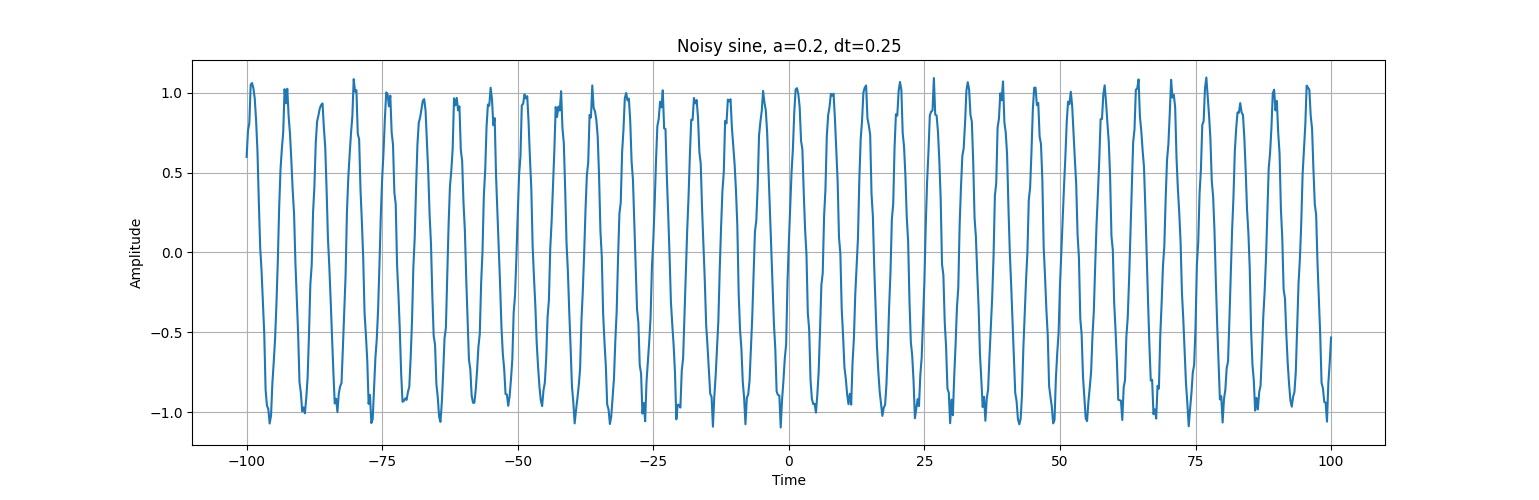
\includegraphics[scale=0.4]{1_noisy_sine.png}
        \captionsetup{skip=0pt}
        \caption{График зашумленного сигнала.}
        \label{fig:1ns}
    \end{figure}
    Найдем численную производную от данного сигнала, используя формулу поэлементного дифференцирования $$\dfrac{y(k+1)-y(k)}{dt},$$ после чего построим график.
    \begin{figure}[H]
        \centering
        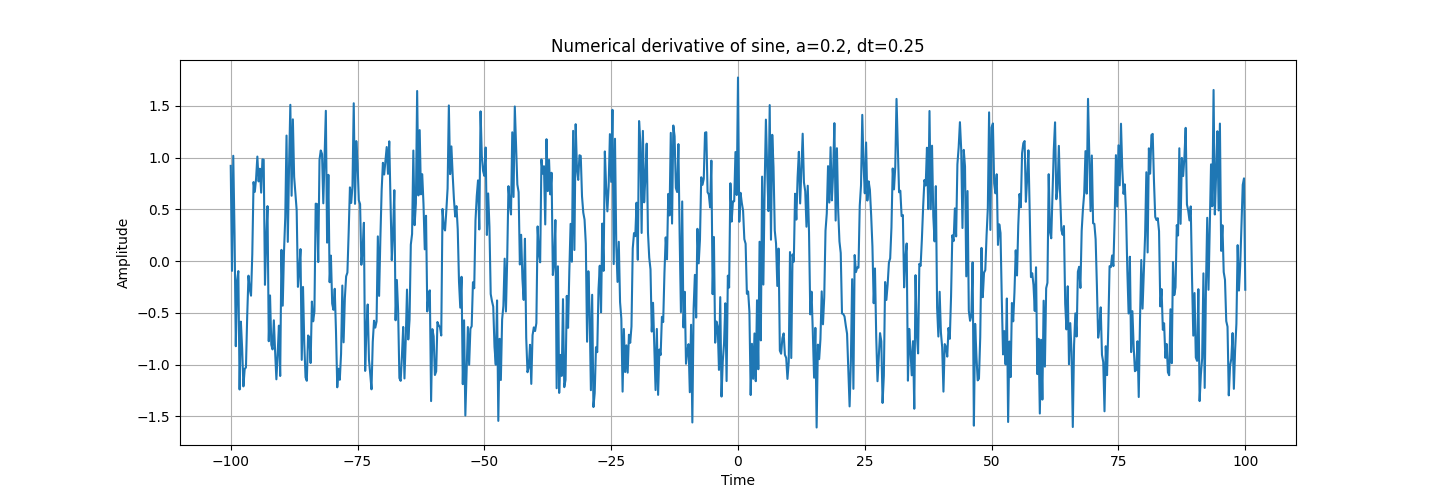
\includegraphics[scale=0.4]{1_numdiff_sine.png}
        \captionsetup{skip=0pt}
        \caption{Численная производная зашумленного сигнала.}
        \label{fig:1nds}
    \end{figure}
    Найдем спектральную производную от зашумленного сигнала. Для прямого и обратного преобразования Фурье будем использовать численное интегрирование (trapz). Чтобы
    превратить Фурье-образ сигнала в Фурье-образ производной, необходимо домножить результат преобразования Фурье на $2\pi i \nu$, где $\nu$ -- частота (Гц),
    таким образом получим формулу $$\mathcal{F}\left\{\frac{d}{dt}f\right\}=2\pi i \nu \mathcal{F}\left\{f\right\}.$$ Теперь остается только выполнить обратное преобразование Фурье, чтобы получить
    спектральную производную сигнала. Далее приведены графики вещественной и мнимой компонент Фурье-образа сигнала и его спектральной производной.
    \begin{figure}[H]
        \centering
        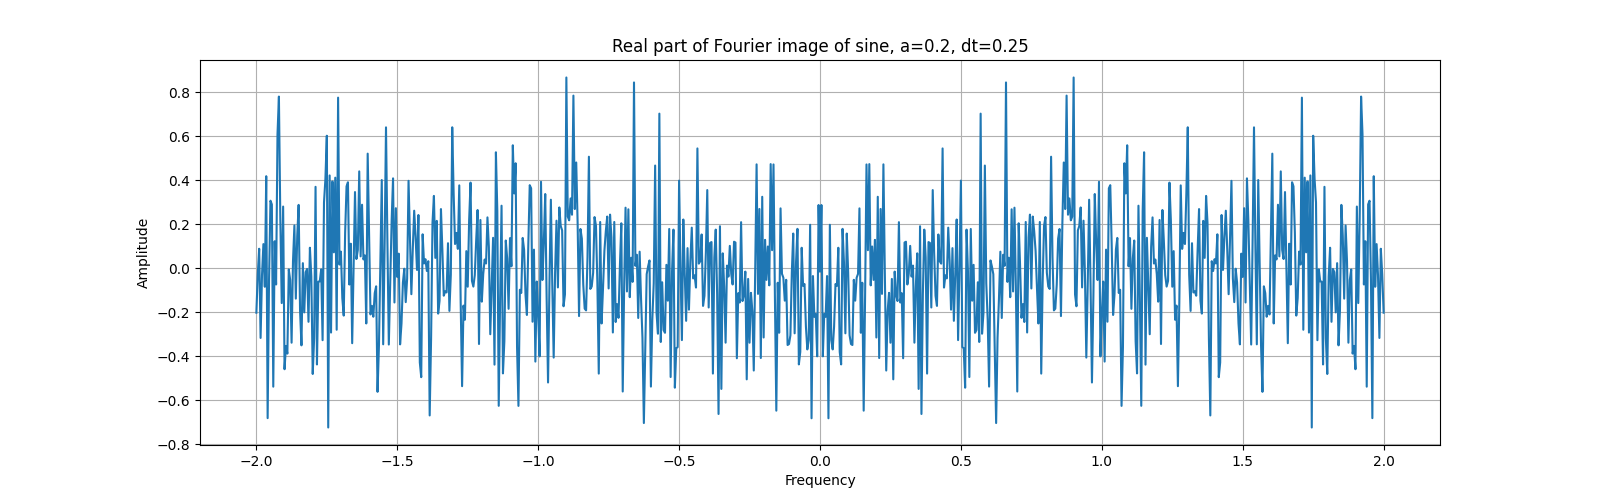
\includegraphics[scale=0.4]{1_re_fimg_sine.png}
        \captionsetup{skip=0pt}
        \caption{Вещественная компонента Фурье-образа зашумленного сигнала.}
        \label{fig:1refis}
    \end{figure}
    \begin{figure}[H]
        \centering
        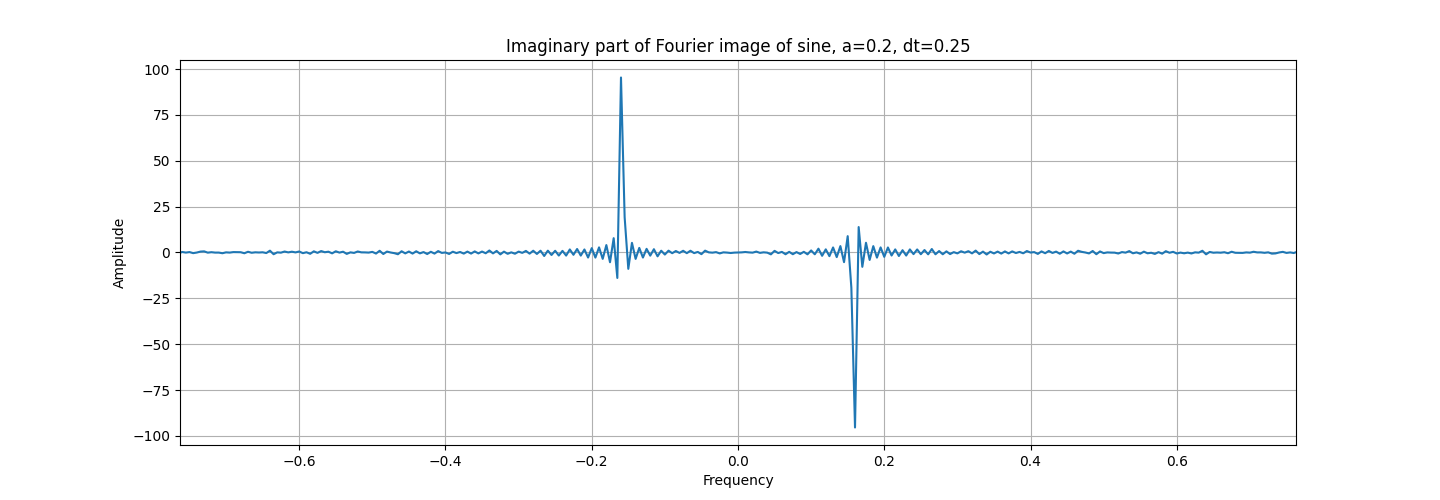
\includegraphics[scale=0.4]{1_im_fimg_sine.png}
        \captionsetup{skip=0pt}
        \caption{Мнимая компонента Фурье-образа зашумленного сигнала.}
        \label{fig:1imfis}
    \end{figure}
    \begin{figure}[H]
        \centering
        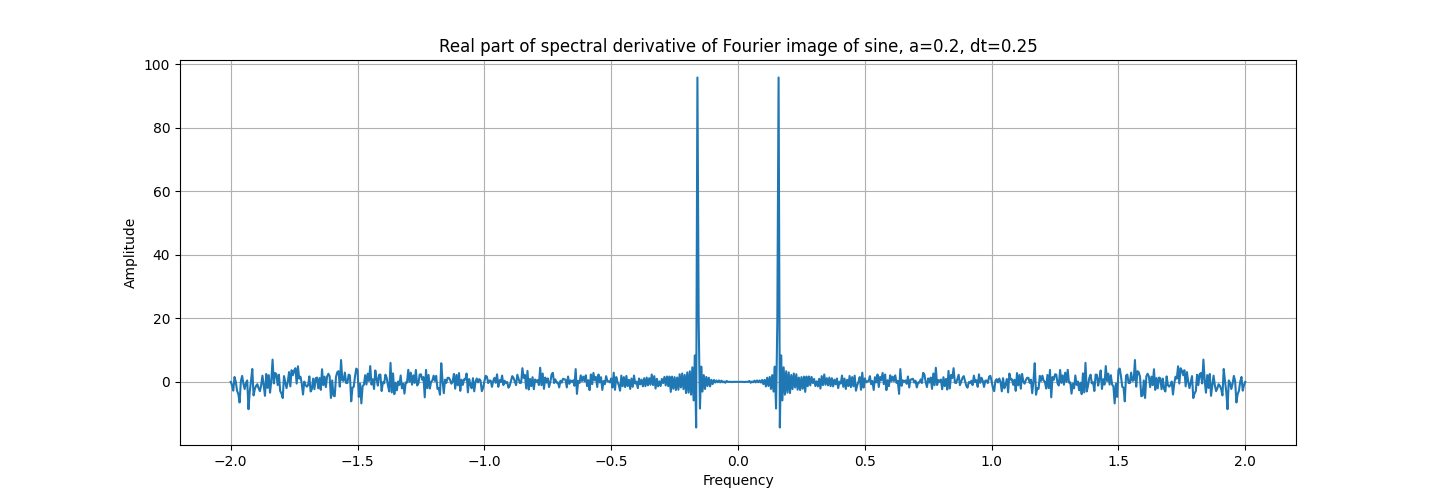
\includegraphics[scale=0.4]{1_re_spd_fimg_sine.png}
        \captionsetup{skip=0pt}
        \caption{Вещественная компонента спектральной производной Фурье-образа зашумленного сигнала.}
        \label{fig:1respdf}
    \end{figure}
    \begin{figure}[H]
        \centering
        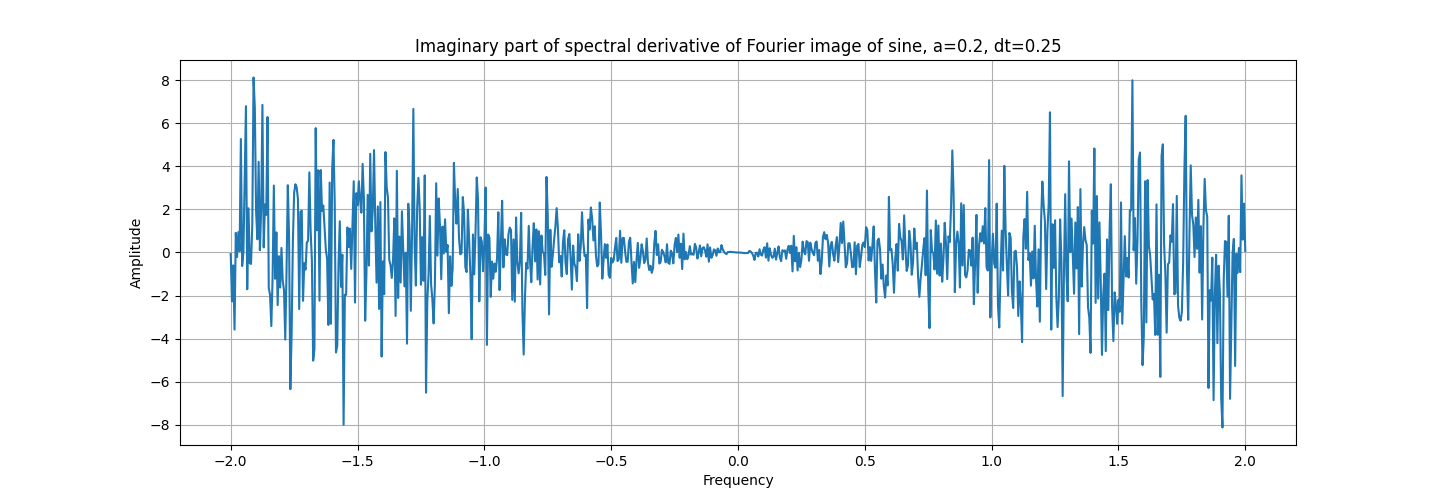
\includegraphics[scale=0.4]{1_im_spd_fimg_sine.png}
        \captionsetup{skip=0pt}
        \caption{Мнимая компонента спектральной производной Фурье-образа зашумленного сигнала.}
        \label{fig:1imspdf}
    \end{figure}


    Видим, что вещественная компонента Фурье-образа зашумленного сигнала и его спектральной производной симметричны относительно оси
    $OY$, а их мнимые компоненты относительно $OX$. Подобная симметричность сохраняется в не зависимости от четности исходной функции.


    На следующем рисунке приведен график вещественной части спектральной производной зашумленного сигнала, найденной с помощью численного интегрирования.
    Результат похож на численную производную, но с резкими возрастаниями амплитуд по краям. Данное поведение не зависит от наличия шума в сигнале или
    выбора шага дискретизации $dt$.
    \begin{figure}[H]
        \centering
        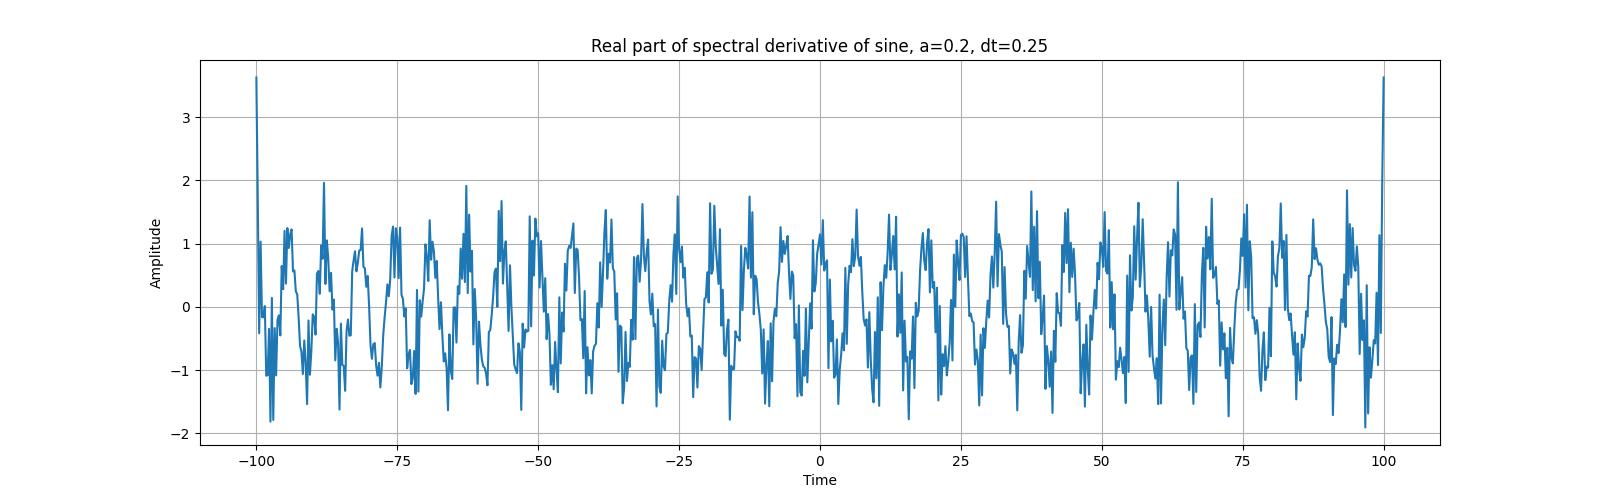
\includegraphics[scale=0.4]{1_re_specdiff_sine.png}
        \captionsetup{skip=0pt}
        \caption{Вещественная компонента спектральной производной зашумленного сигнала.}
        \label{fig:1respds}
    \end{figure}

    
    Теперь сравним график истинной производной $\cos{(t)}$ с графиками численной и спектральной производных зашумленного синуса.
    Оранжевым цветом обозначена спектральная производная, синим численная. Красным цветом выделена производная косинуса.
    \begin{figure}[H]
        \centering
        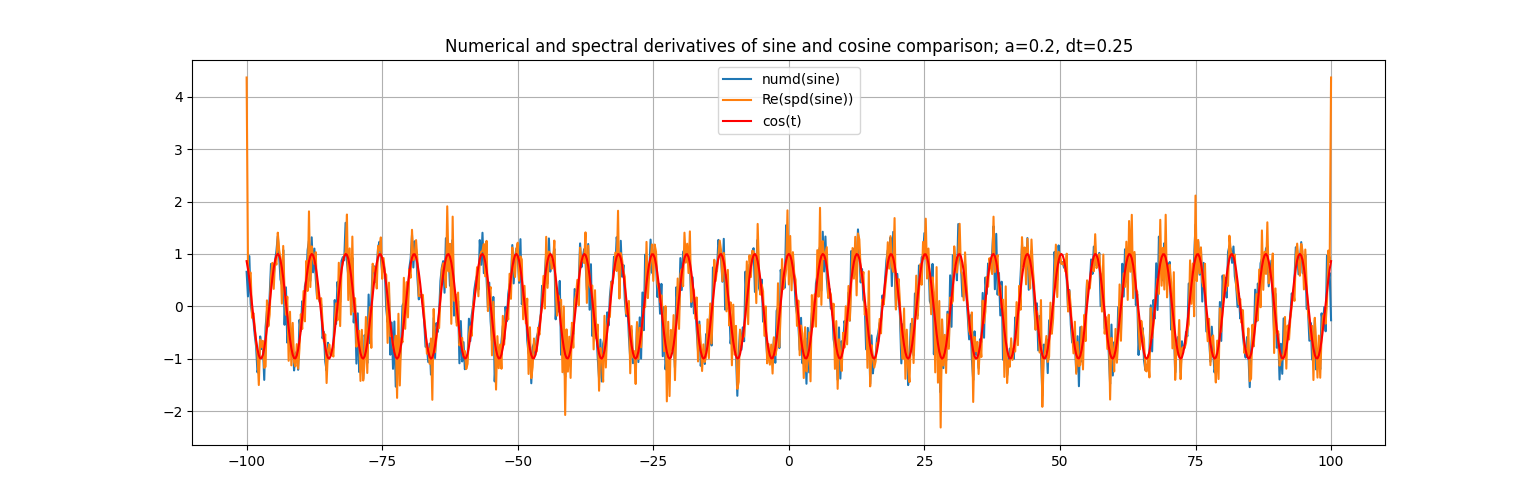
\includegraphics[scale=0.4]{1_css_comp.png}
        \captionsetup{skip=0pt}
        \caption{Сравнительный график $\cos{(t)}$ с численной и спектральной производными зашумленного $\sin{(t)}$.}
        \label{fig:css_comp}
    \end{figure}


    Графики численной и спектральной производных похожи друг на друга и на истинную производную $\cos{(t)}$.
    Спектральная производная имеет немного больше выбросов по сравнению с численной. Достаточно посмотреть
    на края графика спектральной производной и на ее амплитуды в точках максимума и минимума каждой волны.


    В ходе работы было выяснено, что при маленьком шаге $dt$ или при большом значении $a$ спектральная и численная производные
    становятся не похожи на истинную производную косинуса. По большей части на графиках видно белый шум. Если исходный сигнал
    имеет шумы, то его производная будет зашумлена сильнее. Наличие мнимой части у Фурье-образа не зависит от четности исходной
    функции. Более того, вещественные компоненты после преобразования Фурье симметричны относительно оси ординат, а мнимые относительно
    оси абсцисс.


    \subsection{Используемые программы.}
    Все графики перового задания строились с помощью языка программирования Python с подключенной библиотекой matplotlib. Далее
    по ходу работы графики будут строиться той же программой. 
    \begin{lstlisting}[label=task1, caption={Файл с программой для построения графиков.}]
    import matplotlib.pyplot as plt

    def build_f(x, y, fz1=16,
                fz2=5, clr=None, ttl=None,
                grid=True, legend=False, xlab=None,
                ylab=None, xl1=None, xl2=None,
                yl1=None, yl2=None, lbl=None,
                ls='-', ticks=None, rot=None):
        plt.plot(x, y, color=clr, label=lbl, linestyle=ls)
        plt.xlabel(xlab)
        plt.ylabel(ylab)
        plt.xlim(xl1, xl2)
        plt.ylim(yl1, yl2)
        plt.xticks(ticks, rotation=rot)
        plt.title(ttl)
        plt.gcf().set_size_inches(fz1, fz2)
        plt.grid(grid)
        if legend:
            plt.legend()
        plt.show()
                
    def build_fs(x, y: list, colors: list=None,
                 labels: list=None, fz1=16, fz2=5,
                 ttl=None, grid=True, legend=False, 
                 xlab=None, ylab=None, xl1=None,
                 xl2=None, yl1=None, yl2=None,
                 ls:list=None, ticks=None, rot=None):
        if (y is None or len(y) <= 0):
            print('y is None or its len <= 0')
            return
        if (colors is None): colors = [None] * len(y)
        if (labels is None): labels = [None] * len(y)
        if (ls is None): ls = ['-'] * len(y)
        
        for k in range(len(y)):
            plt.plot(x, y[k], color=colors[k],
                     label=labels[k], linestyle=ls[k])
        plt.xlabel(xlab)
        plt.ylabel(ylab)
        plt.xlim(xl1, xl2)
        plt.ylim(yl1, yl2)
        plt.xticks(ticks, rotation=rot)
        plt.title(ttl)
        plt.gcf().set_size_inches(fz1, fz2)
        plt.grid(grid)
        if legend: plt.legend()
        plt.show()
    \end{lstlisting}


    \newpage
    Для нахождения Фурье-образа и производных использовалась библиотека numpy.
    \begin{lstlisting}[label=task1_2, caption={Программа для вычисления Фурье-образа численным интегрированием и производных.}]
    import numpy as np

    def trapz(y, t, v):
        Y = []
        for k in v:
            Y_k = np.trapz(y * np.exp(-1j * 2 * np.pi * k * t), t)
            Y.append(Y_k)
        return Y

    def undo_trapz(Y, t, v):
        y = []
        for k in t:
            y_k = np.trapz(Y * np.exp(1j * 2 * np.pi * k * v), v)
            y.append(y_k)
        return y

    def numerical_diff(y, dt):
        ndiff = []
        for k in range(len(y) - 1):
            ndiff_k = (y[k + 1] - y[k]) / dt
            ndiff.append(ndiff_k)
        return ndiff

    def spectral_diff(y, t, v):
        Y = trapz(y, t, v)
        dY = 2 * np.pi * 1j * v * Y
        spdiff = undo_trapz(dY, t, v)
        return spdiff, Y, dY
    \end{lstlisting}


    Программа, где используются написанные функции и задаются необходимые параметры, расположена ниже.
    \begin{lstlisting}[label=l, caption={Алгоритм, использующий представленные ранее программы.}]
    import numpy as np

    import build_func as bf
    import fourier_math as fm
    import helper as hr

    T, dt = 200, 0.25
    t = np.arange(-T / 2, T / 2 + dt, dt)
    y = np.sin(t)

    a = 0.2
    y = hr.apply_noise(y, a, t)

    ndsin = fm.numerical_diff(y, dt)
    ndsin.append(y[-1] / 2)

    V, dv = 1 / dt, 1 / T
    v = np.arange(-V / 2, V / 2 + dv, dv)
    spdsin, Y, dY = fm.spectral_diff(y, t, v)
    tdcos = -np.sin(t)

    # Usage example
    bf.build_f(t,
            y,
            ttl=f'Noisy sine, a={a}, dt={dt}',
            xlab='Time',
            ylab='Amplitude')
    bf.build_f(v,
            np.array(Y).real,
            ttl=f'Real part of Fourier image of sine, a={a}, dt={dt}',
            xlab='Frequency',
            ylab='Amplitude')
    bf.build_f(v,
            np.array(Y).imag,
            ttl=f'Imaginary part of Fourier image of sine, a={a}, dt={dt}',
            xlab='Frequency',
            ylab='Amplitude',
            xl1=-0.763,
            xl2=0.763)
    bf.build_fs(
        t,
        y=[ndsin, np.array(spdsin).real, tdcos],
        colors=[None, None, 'r'],
        legend=True,
        labels=[
            'Num. der. of sine', 'Re. spec. der. of sine', 'True der. of cosine'
        ],
        ttl=
        f'True der. of cosine, num. der. of sine and spec. der. of sine comparison; a={a}, dt={dt}'
    )
    \end{lstlisting}


    \section{Задание 2. Линейные фильтры.}
    Рассмотрим сигнал вида $$u=g+b\cdot(\text{random}(\text{len}(t))-0.5) + c\cdot \sin(d\cdot t),$$ который будем пропускать
    через линейные фильтры.


    \subsection{Фильтр первого порядка.}
    Положим $c=0,\,a=1,\,b=0.6,\,d=0.7$. Будем задавать различные значения постоянной времени $T>0$ и пропускать сигнал через линейный
    фильтр первого порядка $$W_1(p)=\dfrac{1}{Tp+1},$$ после чего построим сравнительные графики и исследуем влияние параметров $T$ и $a$
    на эффективность фильтрации.


    Далее расположены сравнительные графики исходного и фильтрованного сигналов, графики модулей их Фурье-образов, а также АЧХ и ЛАЧХ фильтра.
    В названии графиков указаны значения используемых параметров. Синим цветом обозначаются функции, относящиеся к исходному сигналу, оранжевым
    -- к фильтрованному. Дополнительно на графике во временной области отрисована исходная функция $g(t)$ для более наглядного рассмотрения работы
    фильтрации.
    \begin{figure}[H]
        \centering
        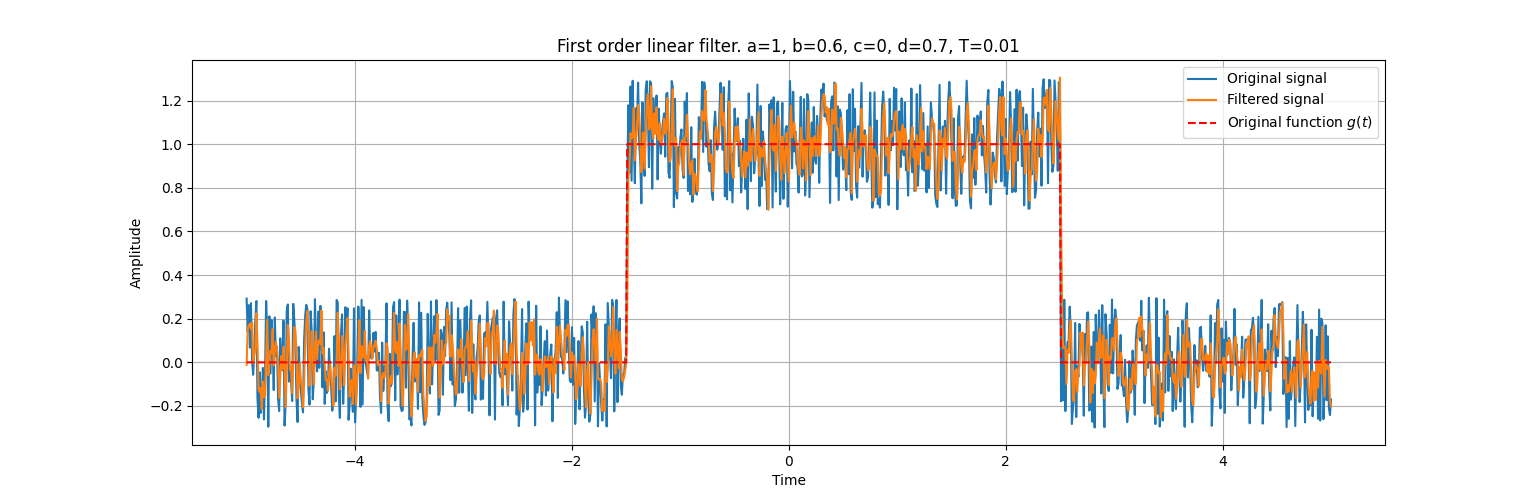
\includegraphics[scale=0.4]{1_filtered_linear.png}
        \captionsetup{skip=0pt}
        \caption{График исходного и фильтрованного сигналов (1).}
        \label{fig:filin1}
    \end{figure}
    \begin{figure}[H]
        \centering
        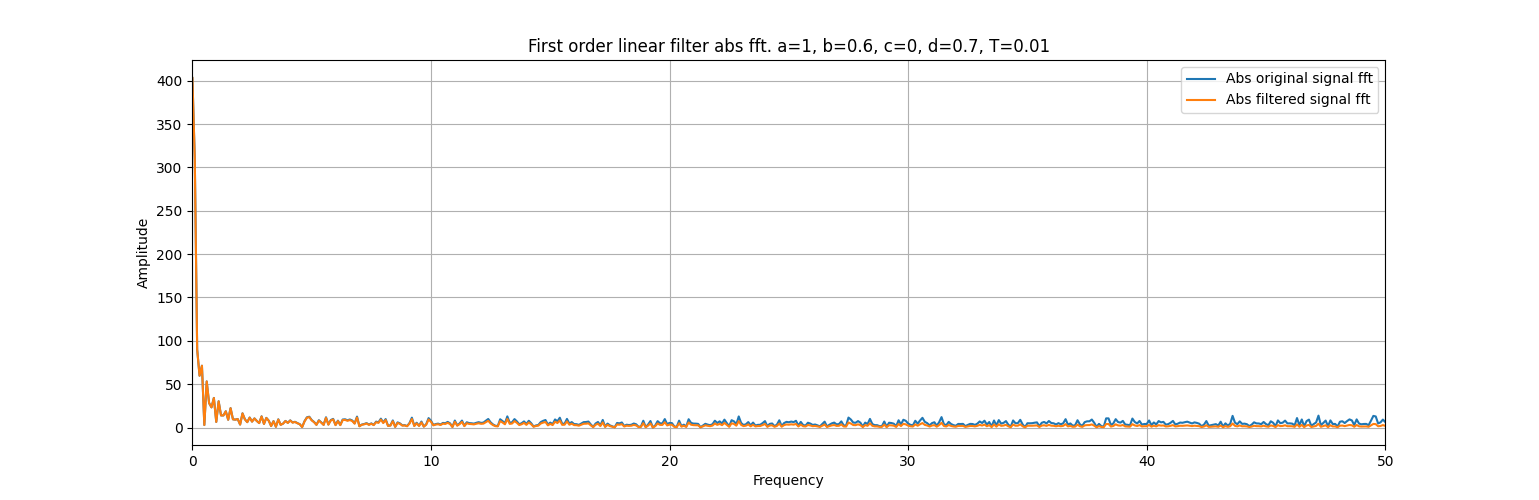
\includegraphics[scale=0.4]{1_abs_filtered_linear.png}
        \captionsetup{skip=0pt}
        \caption{График модулей Фурье-образа исходного и фильтрованного сигналов (1).}
        \label{fig:filinabs1}
    \end{figure}
    \begin{figure}[H]
        \centering
        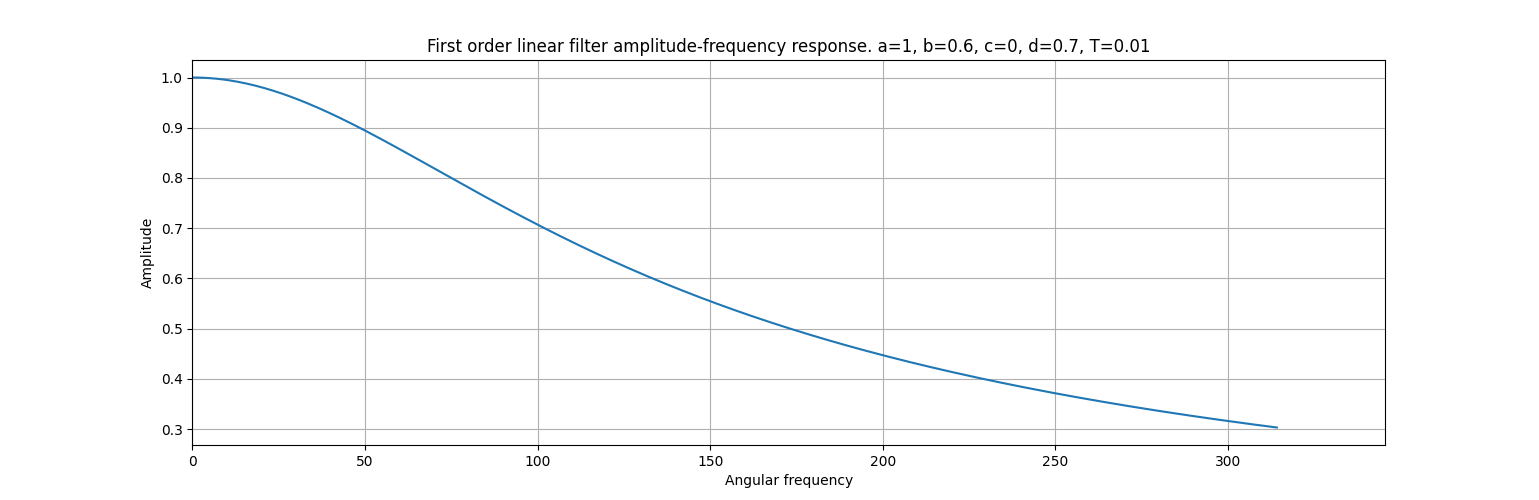
\includegraphics[scale=0.4]{1_afr_filtered_linear.png}
        \captionsetup{skip=0pt}
        \caption{График амплитудно-частотной характеристики фильтра (1).}
        \label{fig:filinafr1}
    \end{figure}
    \begin{figure}[H]
        \centering
        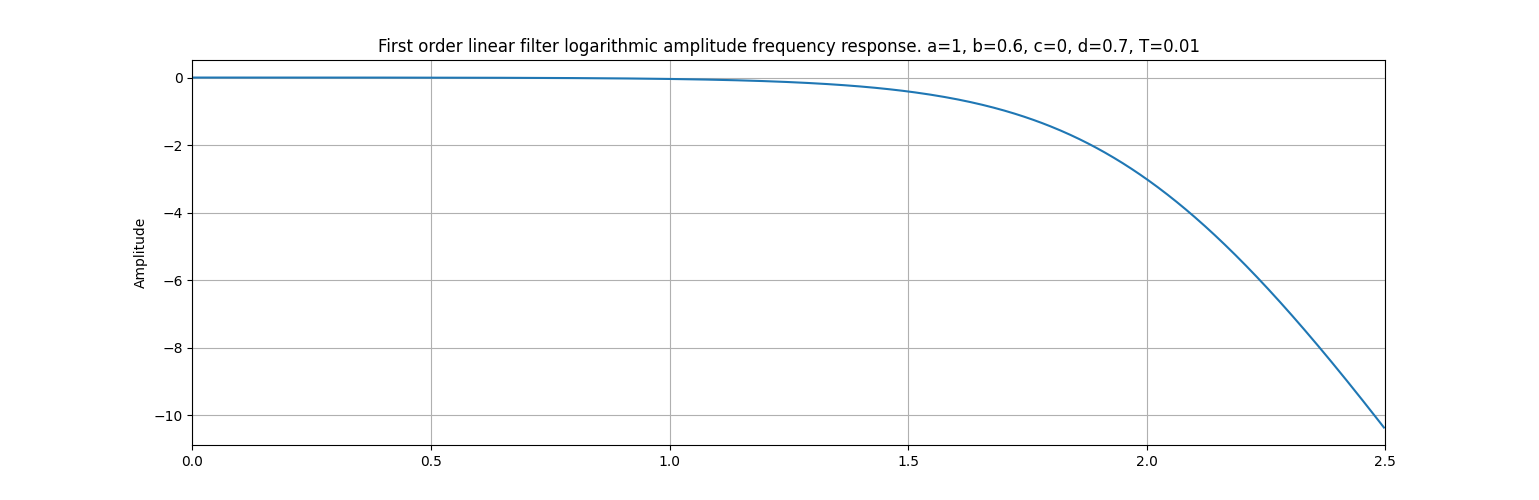
\includegraphics[scale=0.4]{1_lafr_filtered_linear.png}
        \captionsetup{skip=0pt}
        \caption{График логарифмической амплитудно-частотной характеристики фильтра (1).}
        \label{fig:filinlafr1}
    \end{figure}
    \begin{figure}[H]
        \centering
        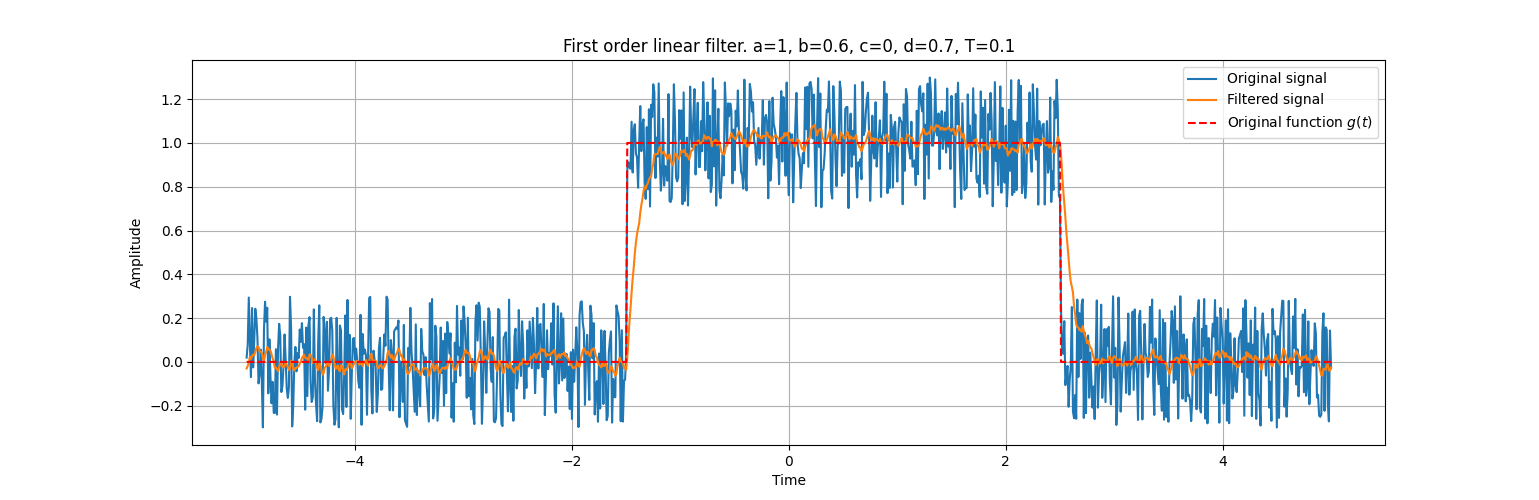
\includegraphics[scale=0.4]{2_filtered_linear.png}
        \captionsetup{skip=0pt}
        \caption{График исходного и фильтрованного сигналов (2).}
        \label{fig:filin11}
    \end{figure}
    \begin{figure}[H]
        \centering
        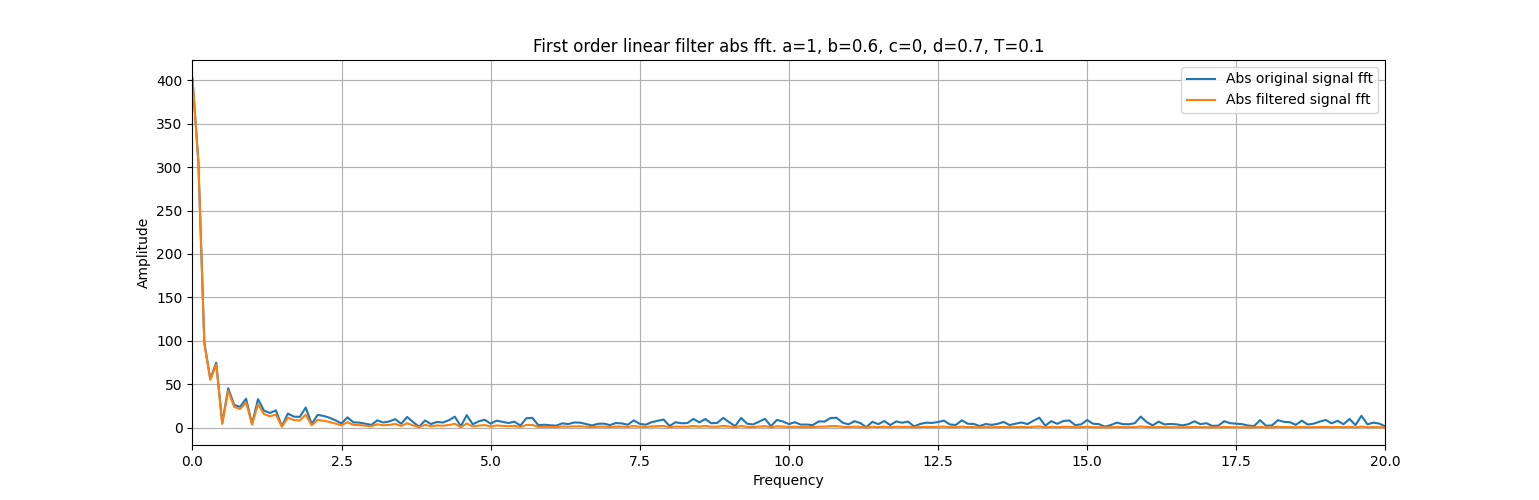
\includegraphics[scale=0.4]{2_abs_filtered_linear.png}
        \captionsetup{skip=0pt}
        \caption{График модулей Фурье-образа исходного и фильтрованного сигналов (2).}
        \label{fig:filinabs11}
    \end{figure}
    \begin{figure}[H]
        \centering
        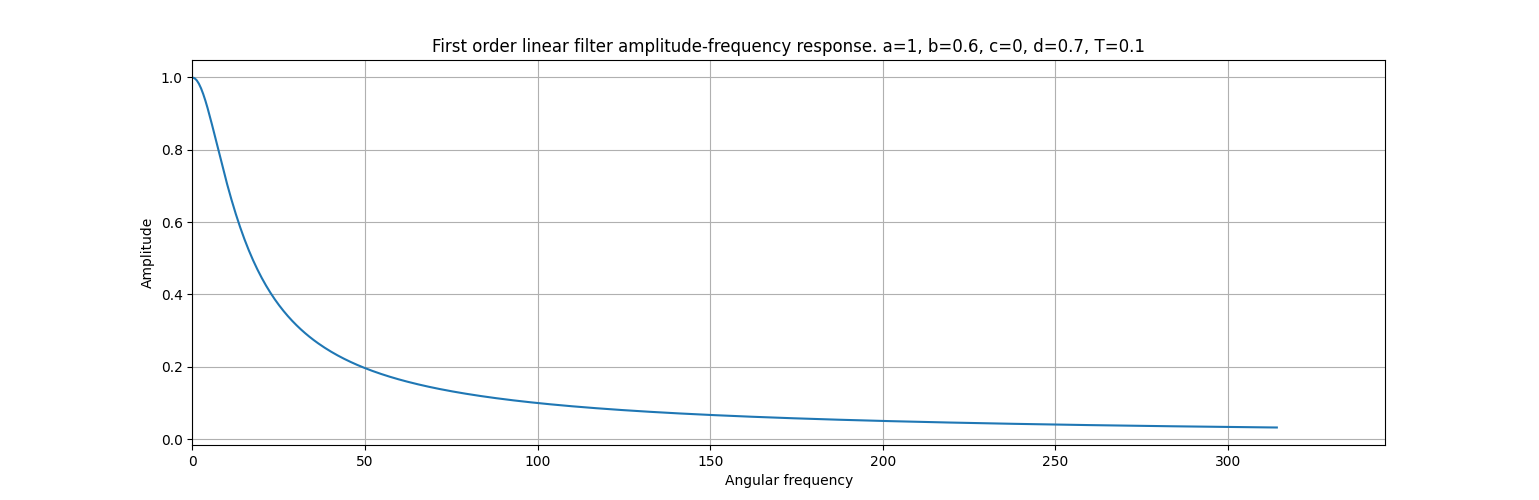
\includegraphics[scale=0.4]{2_afr_filtered_linear.png}
        \captionsetup{skip=0pt}
        \caption{График амплитудно-частотной характеристики фильтра (2).}
        \label{fig:filinafr11}
    \end{figure}
    \begin{figure}[H]
        \centering
        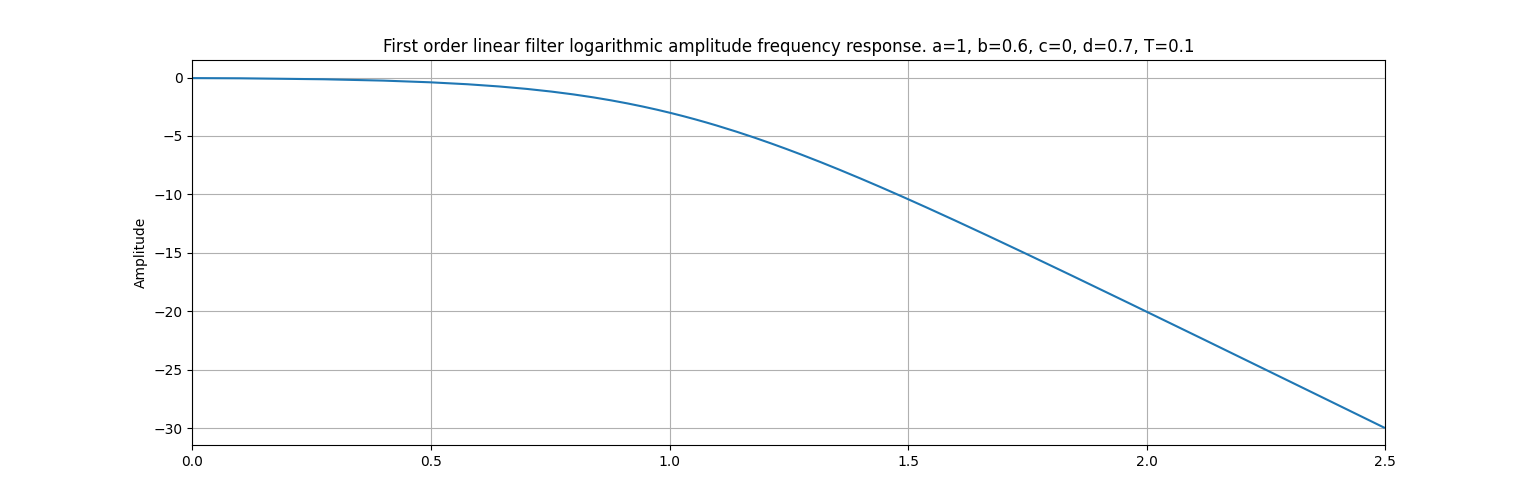
\includegraphics[scale=0.4]{2_lafr_filtered_linear.png}
        \captionsetup{skip=0pt}
        \caption{График логарифмической амплитудно-частотной характеристики фильтра (2).}
        \label{fig:filinlafr11}
    \end{figure}
    \begin{figure}[H]
        \centering
        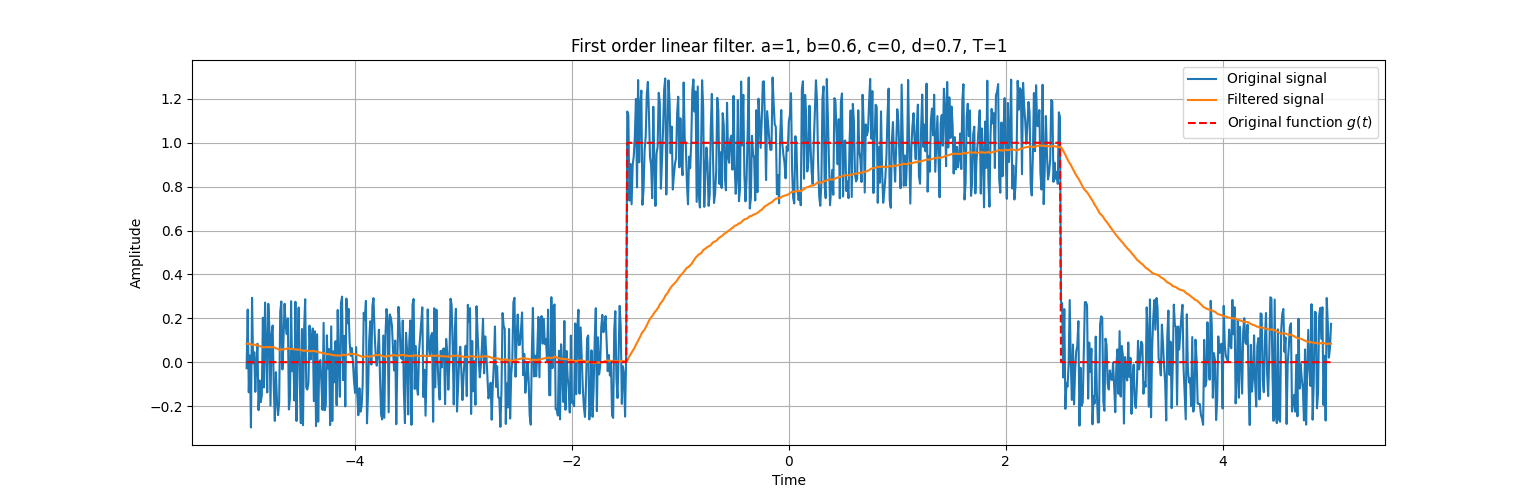
\includegraphics[scale=0.4]{3_filtered_linear.png}
        \captionsetup{skip=0pt}
        \caption{График исходного и фильтрованного сигналов (3).}
        \label{fig:filin13}
    \end{figure}
    \begin{figure}[H]
        \centering
        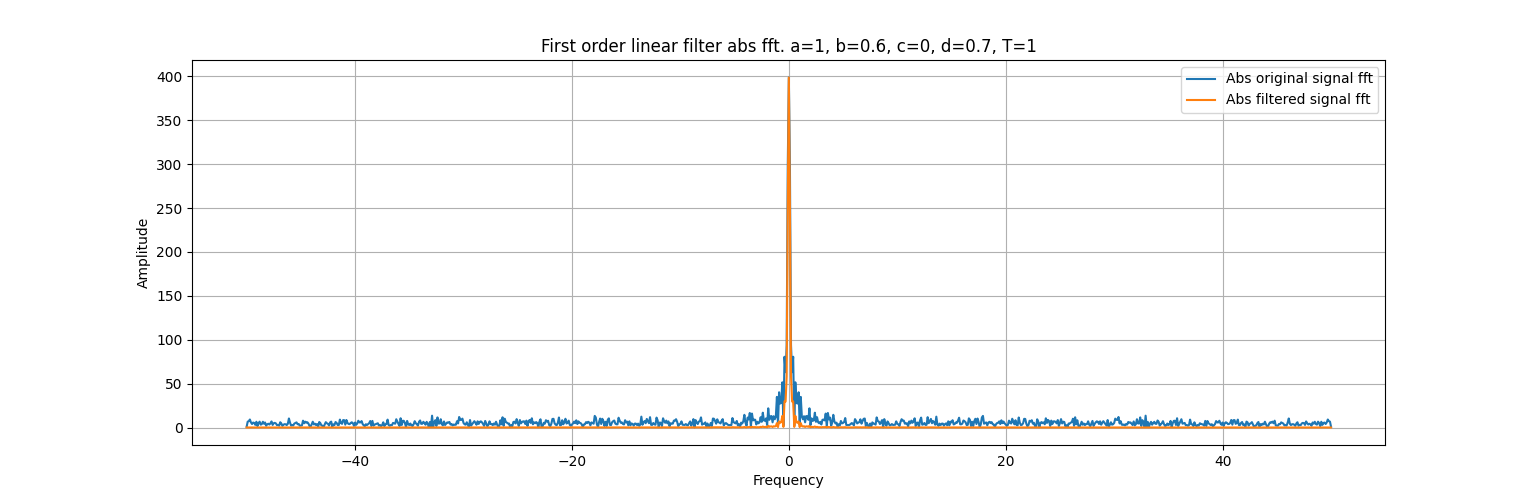
\includegraphics[scale=0.4]{3_abs_filtered_linear.png}
        \captionsetup{skip=0pt}
        \caption{График модулей Фурье-образа исходного и фильтрованного сигналов (3).}
        \label{fig:filinabs13}
    \end{figure}
    \begin{figure}[H]
        \centering
        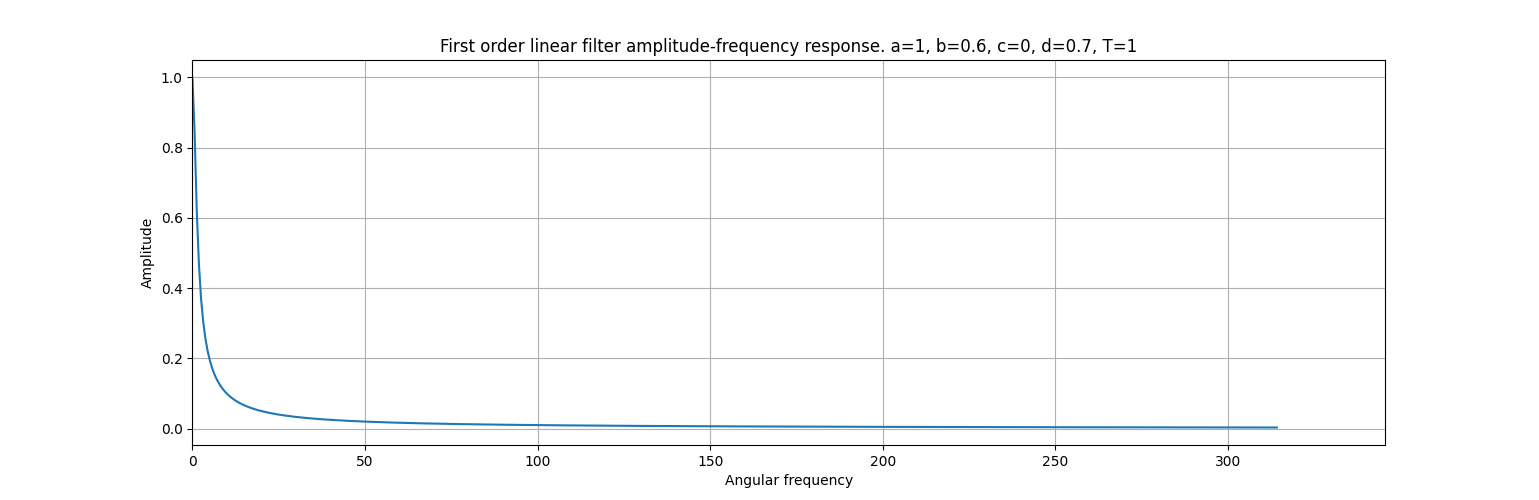
\includegraphics[scale=0.4]{3_afr_filtered_linear.png}
        \captionsetup{skip=0pt}
        \caption{График амплитудно-частотной характеристики фильтра (3).}
        \label{fig:filinafr13}
    \end{figure}
    \begin{figure}[H]
        \centering
        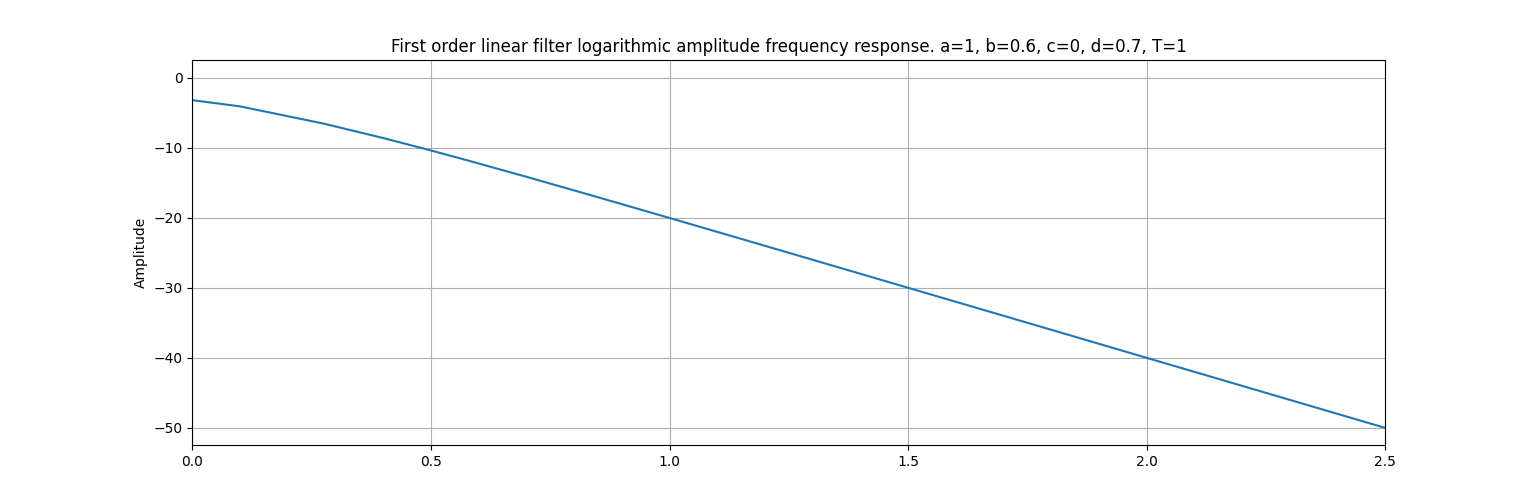
\includegraphics[scale=0.4]{3_lafr_filtered_linear.png}
        \captionsetup{skip=0pt}
        \caption{График логарифмической амплитудно-частотной характеристики фильтра (3).}
        \label{fig:filinlafr13}
    \end{figure}
    \begin{figure}[H]
        \centering
        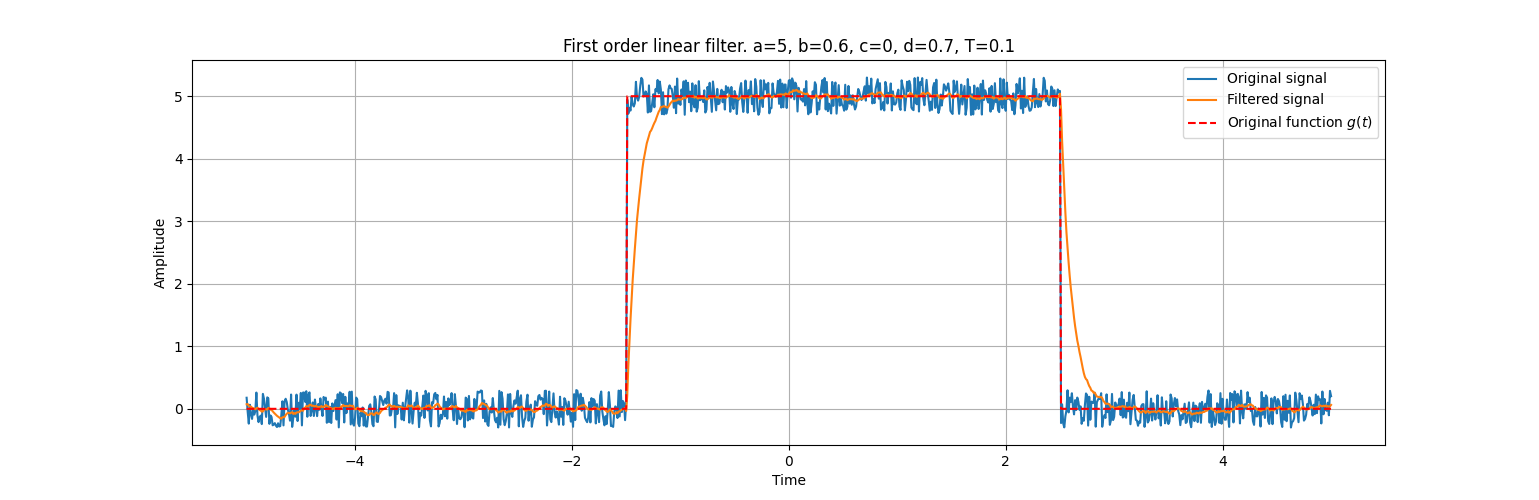
\includegraphics[scale=0.4]{4_filtered_linear.png}
        \captionsetup{skip=0pt}
        \caption{График исходного и фильтрованного сигналов (4).}
        \label{fig:filin14}
    \end{figure}
    \begin{figure}[H]
        \centering
        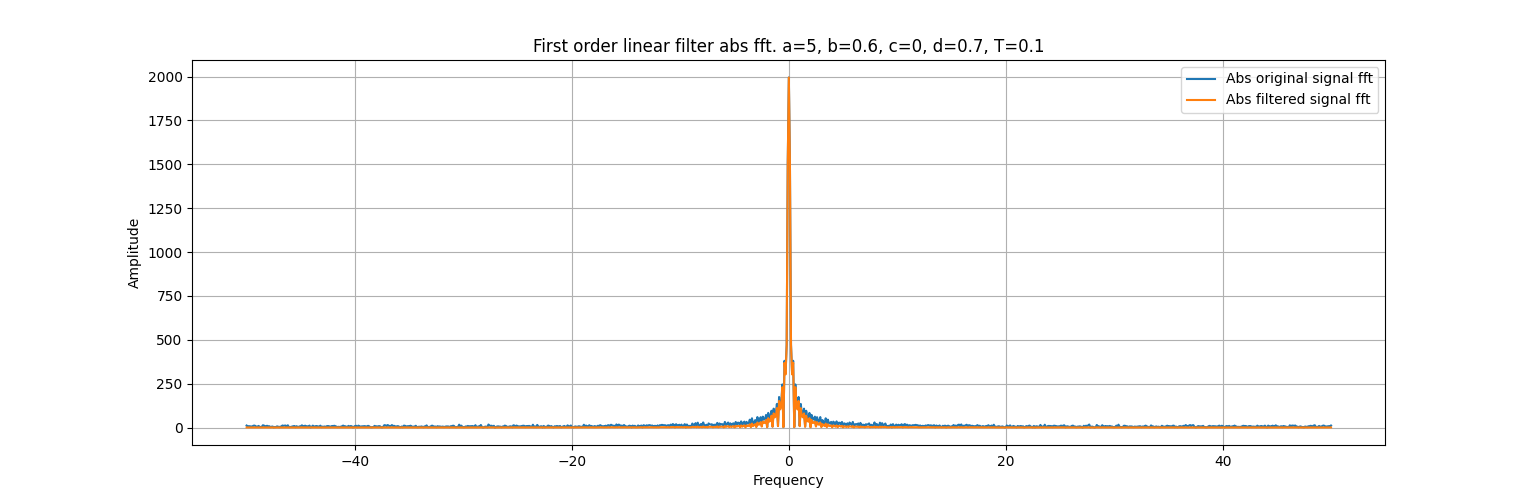
\includegraphics[scale=0.4]{4_abs_filtered_linear.png}
        \captionsetup{skip=0pt}
        \caption{График модулей Фурье-образа исходного и фильтрованного сигналов (4).}
        \label{fig:filinabs14}
    \end{figure}
    \begin{figure}[H]
        \centering
        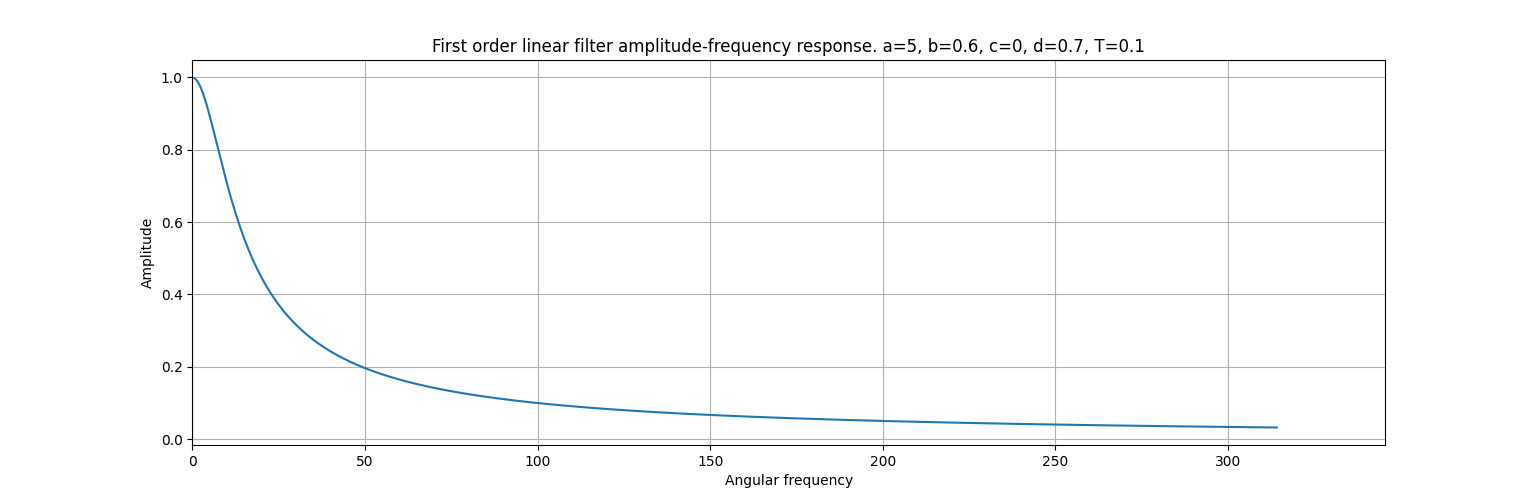
\includegraphics[scale=0.4]{4_afr_filtered_linear.png}
        \captionsetup{skip=0pt}
        \caption{График амплитудно-частотной характеристики фильтра (4).}
        \label{fig:filinafr14}
    \end{figure}
    \begin{figure}[H]
        \centering
        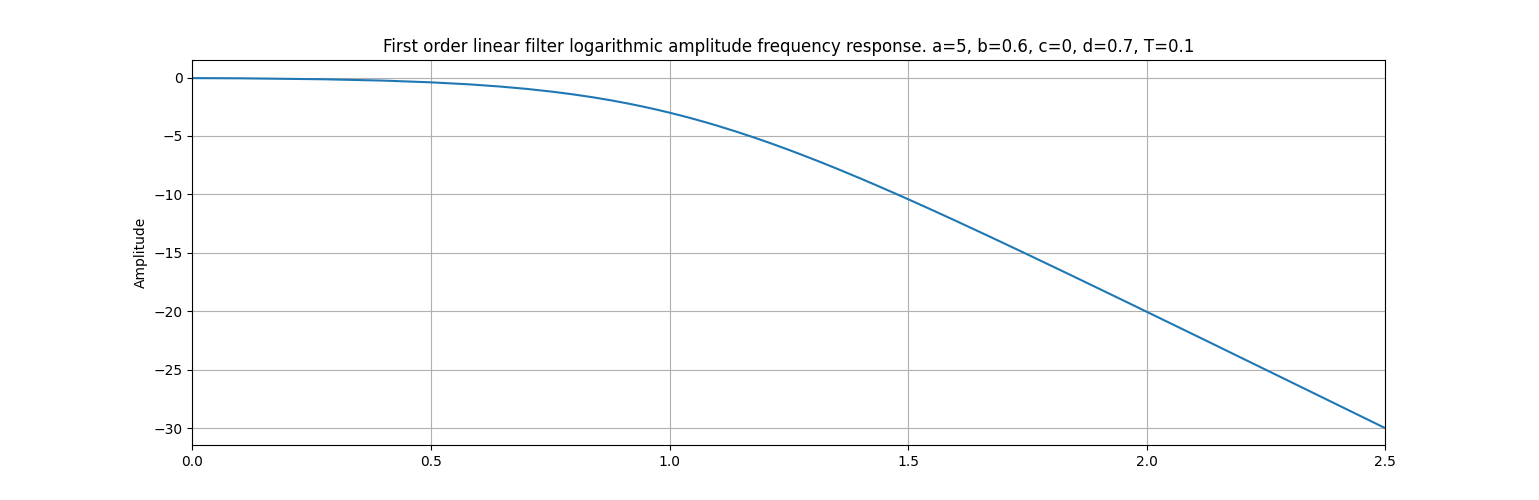
\includegraphics[scale=0.4]{4_lafr_filtered_linear.png}
        \captionsetup{skip=0pt}
        \caption{График логарифмической амплитудно-частотной характеристики фильтра (4).}
        \label{fig:filinlafr14}
    \end{figure}
    \begin{figure}[H]
        \centering
        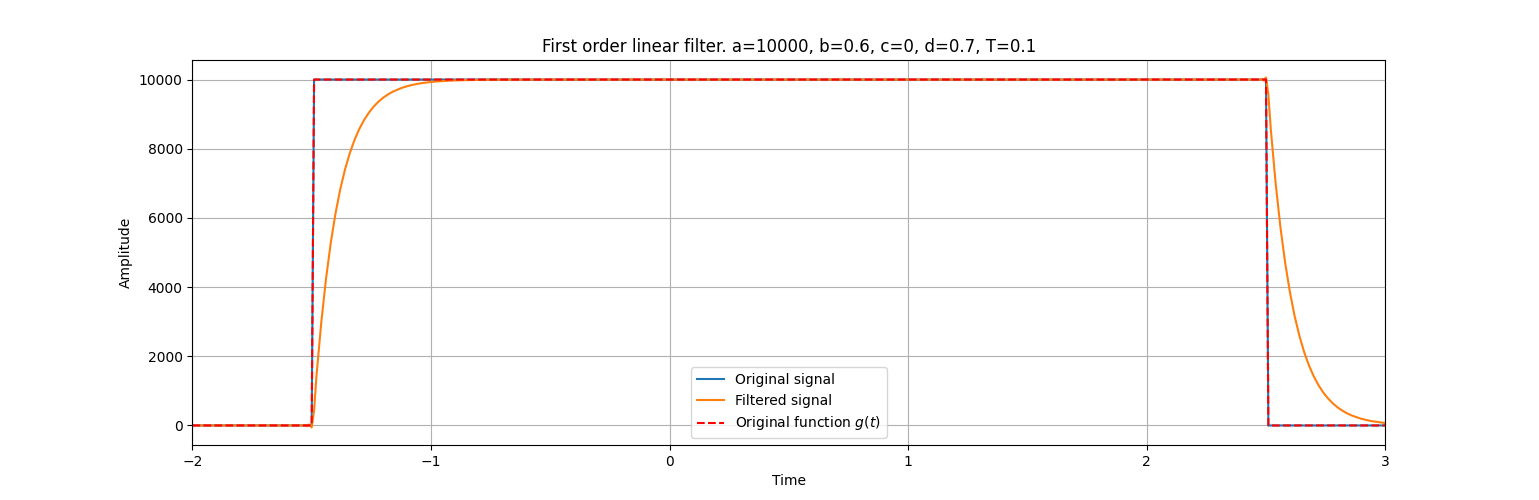
\includegraphics[scale=0.4]{alin1.png}
        \captionsetup{skip=0pt}
        \caption{Более детальное исследование параметра $a$ (Исходный и фильтрованный сигнал).}
        \label{fig:alin1}
    \end{figure}
    \begin{figure}[H]
        \centering
        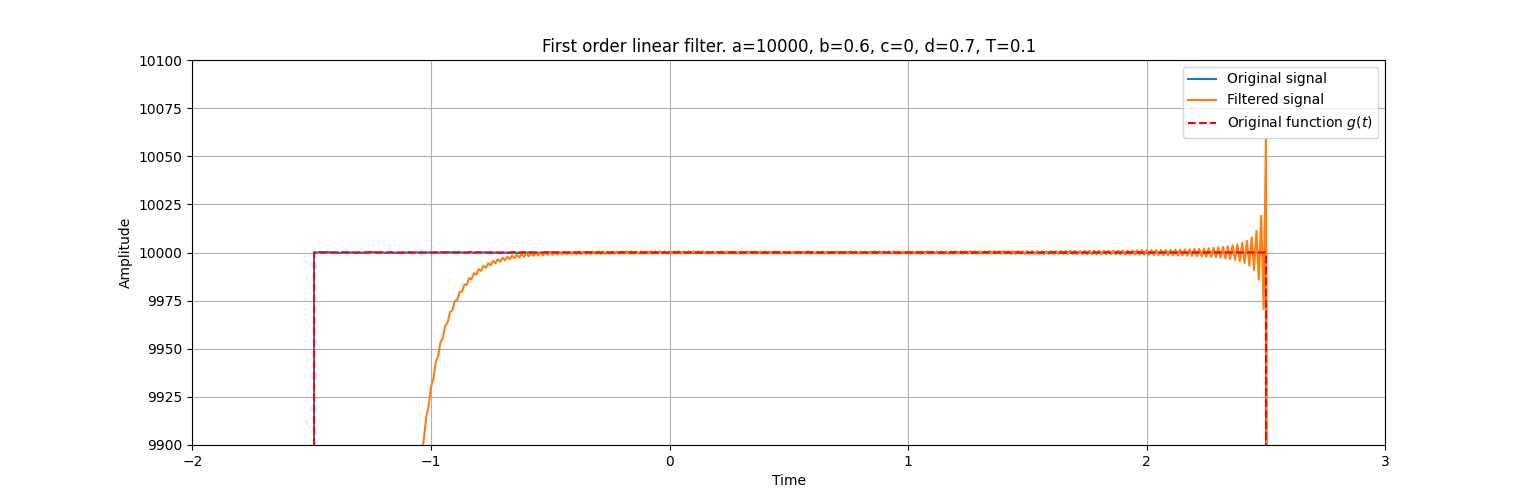
\includegraphics[scale=0.4]{alin2.png}
        \captionsetup{skip=0pt}
        \caption{Более детальное исследование параметра $a$ (Поднятая часть сигналов в приближении).}
        \label{fig:alin2}
    \end{figure}
    \begin{figure}[H]
        \centering
        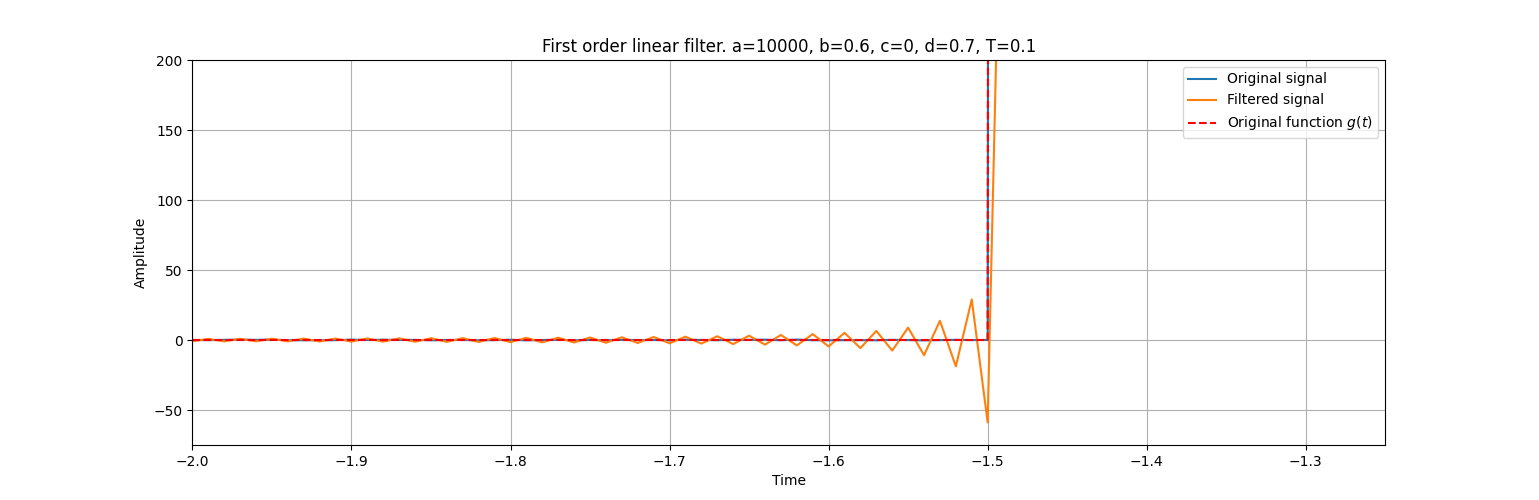
\includegraphics[scale=0.4]{alin3.png}
        \captionsetup{skip=0pt}
        \caption{Более детальное исследование параметра $a$ (Левый разрыв сигналов).}
        \label{fig:alin3}
    \end{figure}
    \begin{figure}[H]
        \centering
        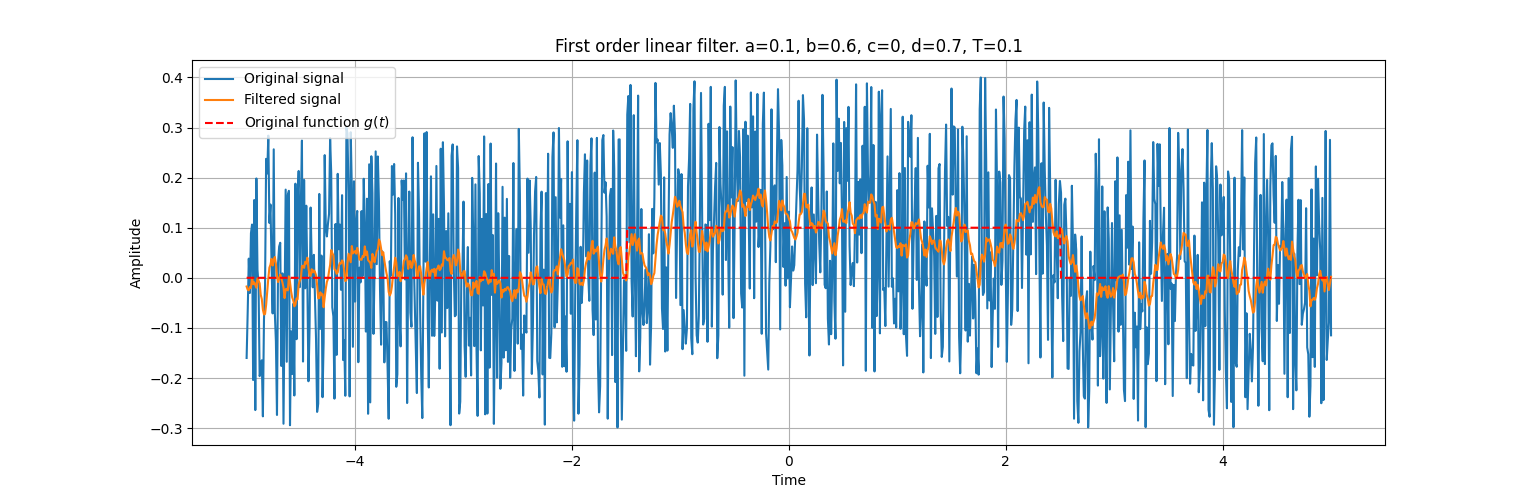
\includegraphics[scale=0.4]{alin4.png}
        \captionsetup{skip=0pt}
        \caption{Более детальное исследование параметра $a$.}
        \label{fig:alin4}
    \end{figure}


    Исходя из графиков можно сделать вывод, что при маленьких и больших значениях постоянной времени $T$ фильтрация хуже,
    чем при средних значениях. Большие значения приводят к излишей фильтрации сигнала -- результирующий сигнал хоть и хорошо
    сглажен, но приобрел лишний наклон (см. рис. \ref{fig:filin13}). На рис. \ref{fig:filinabs13} видно, что в некотором
    небольшом диапазоне нуля большинство важных частот (имеющих б\'{о}льшие амплитуды по сравнению с другими) урезалось
    фильтром. Еще лучше это видно на графике АЧХ -- частота среза по оси абсцисс находится близко к оси ординат, что означает,
    что фильтр оставил немного амплитуд, соответствующих нижним частотам, нетронутыми, а ниже частоты среза график быстро убывает
    -- происходит резкое ослабление амплитуд соответствующих частот (см. рис. \ref{fig:filinafr13}). Маленькие значения приводят к
    недостаточной фильтрации сигнала -- хотя фильтрованный сигнал и выглядит лучше исходного, осталось много белого шума
    (см. рис. \ref{fig:filin1}). На графике модулей Фурье-образов большинство менее значимых частот было оставлено
    (см. рис. \ref{fig:filinabs1}). На графике АЧХ рисунка \ref{fig:filinafr1} хорошо видно, что частота среза
    находится примерно в точке $\left(\omega_0=100,\,A=1\div\sqrt{2}\right)$, и, ослабление амплитуд ниже такой частоты среза несильное
    (график медленно убывает). На графике ЛАЧХ частота среза находится примерно в точке $\left(2,\,-3\right)$ (см. рис. \ref{fig:filinlafr1}).
    На графиках ЛАЧХ (см. рис. \ref{fig:filinlafr1}, \ref{fig:filinlafr11}, \ref{fig:filinlafr13})
    при последовательном увеличении значения $T$ с каждым разом частота среза приближается к нижним частотам, уменьшаясь в 10 раз при
    переводе из логарифмической шкалы частот (изменение на 1 на логарифмической шкале частот соответствует изменению частоты в 10 раз).
    Примерно это мы и видим на графиках АЧХ -- рис. \ref{fig:filinafr1} $\omega_0\approx 100$, рис. \ref{fig:filinafr11} $\omega_0\approx 10$,
    рис. \ref{fig:filinafr13} $\omega_0\approx 1$. Хорошо фильтрация получилась на рис. \ref{fig:filin11} -- большая часть белого шума пропала,
    график не сильно отклонился и неплохо повторяет функцию $g(t)$.
    
    
    Рассматривая рисунки \ref{fig:filin11}, \ref{fig:filin14} и \ref{fig:alin1} кажется, что
    влияние параметра $a$ на эффективность фильтрации заключается в ее сглаживании -- чем больше значение $a$, тем более гладким становится фильтрованный сигнал.
    Однако по рис. \ref{fig:alin2} и \ref{fig:alin3} можно увидеть, что при большом значении $a$ усиливается эффект Гиббса в местах разрыва сигнала, при этом
    чем ближе сигнал к месту разрыва, тем постепенно больше становятся амплитуды фильтрованного сигнала -- фильтрация явно ухудшается. Также при слишком маленьком
    значении параметра $a$ фильтрованный сигнал выглядит хуже при том же значении параметра $T$ (см. рис. \ref{fig:alin4}, \ref{fig:filin11}). Следовательно, параметр
    $a$ так же как и параметр $T$ следует выбирать не маленьким и не большим.


    \subsection{Специальный фильтр.}
    Положим $b=0$. Рассмотрим линейный фильтр вида
    $$W_2(p)=\dfrac{\left(T_1p+1\right)^{2}}{\left(T_2p+1\right)\left(T_3p+1\right)}=\dfrac{T_1^2p^2+2T_1p+1}{T_2T_3p^2+\left(T_2+T_3\right)p+1},$$
    при этом постараемся подобрать такие $T_1,T_2,T_3>0$, чтобы они по возможности хорошо убирали синусоидальную составляющую помехи и не сильно искажали
    полезный сигнал. Также рассмотрим несколько значений параметра $d$ и найдем подходящие $T_1,T_2,T_3$ для каждого случая. После построим сравнительные
    графики и проанализируем влияние параметра $c$ на эффективность фильтрации.


    Далее расположены сравнительные графики исходного и фильтрованного сигналов, графики модулей их Фурье-образов и АЧХ и ЛАЧХ фильтра.
    Синим цветом отрисованы функции, связанные с исходным сигналом, оранжевым -- с фильтрованным. Также на графике во временной области
    отображена исходная функция $g(t)$.
    \begin{figure}[H]
        \centering
        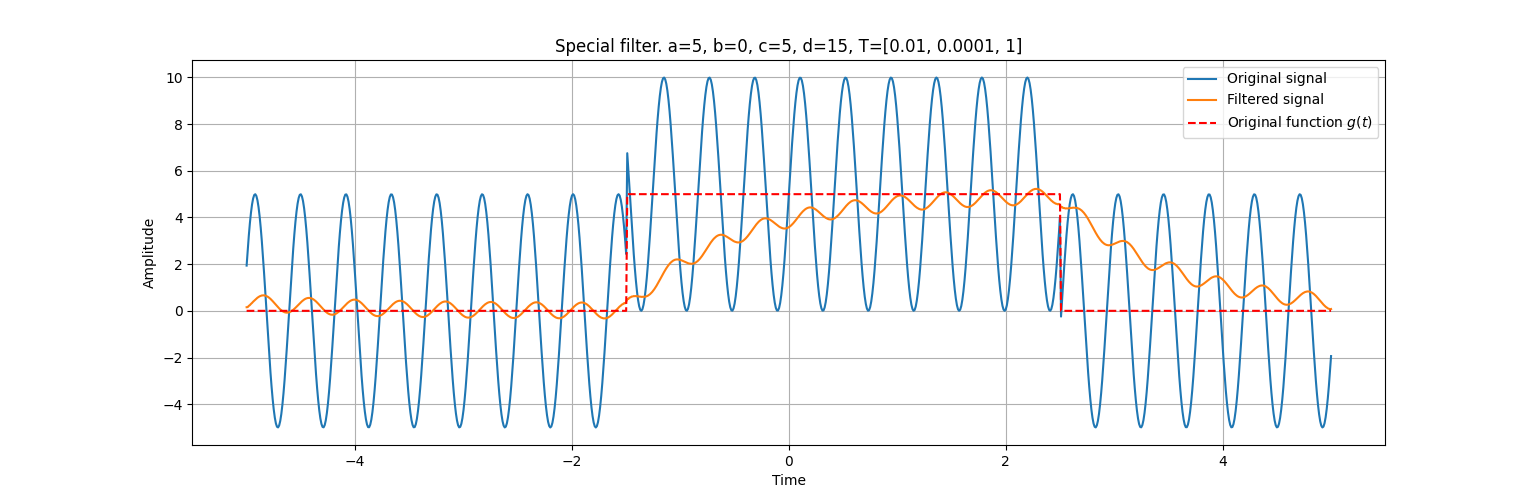
\includegraphics[scale=0.4]{1_fl2.png}
        \captionsetup{skip=0pt}
        \caption{График исходного и фильтрованного сигналов (1).}
        \label{fig:filin21}
    \end{figure}
    \begin{figure}[H]
        \centering
        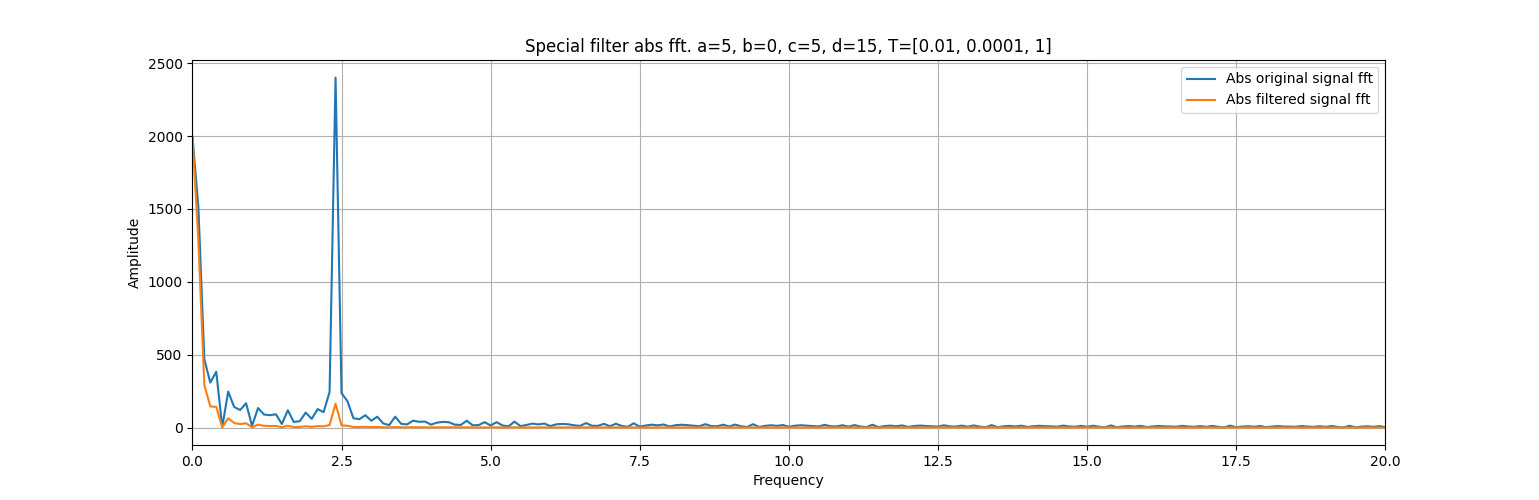
\includegraphics[scale=0.4]{1_fl2_abs.png}
        \captionsetup{skip=0pt}
        \caption{График модулей Фурье-образа исходного и фильтрованного сигналов (1).}
        \label{fig:filinabs21}
    \end{figure}
    \begin{figure}[H]
        \centering
        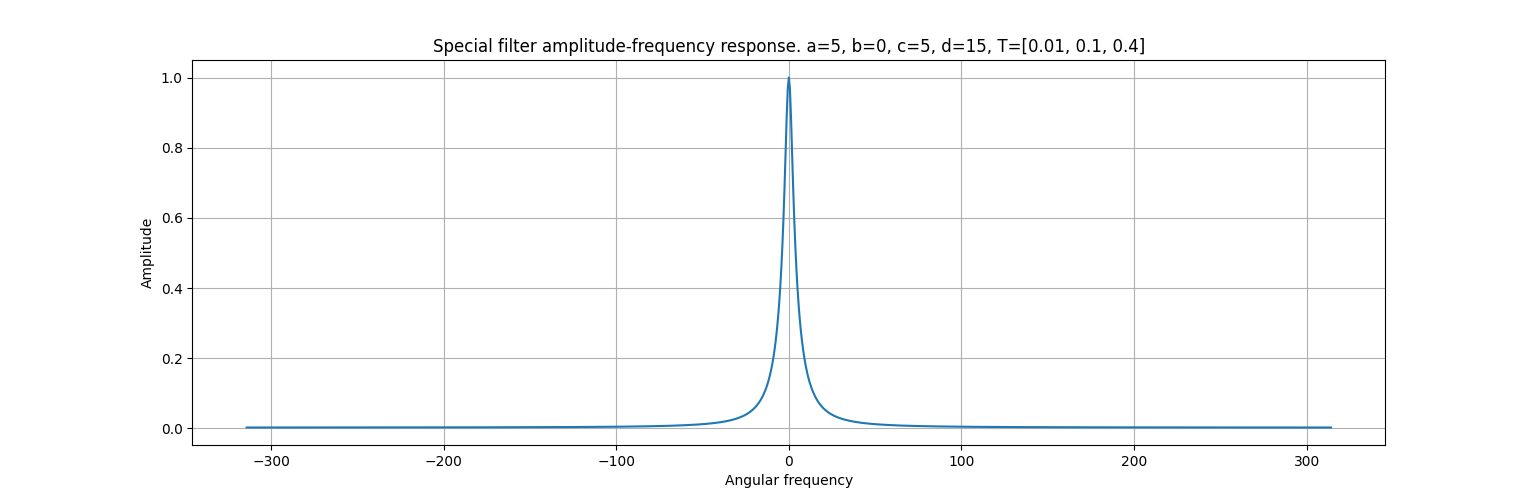
\includegraphics[scale=0.4]{1_fl2_afr.png}
        \captionsetup{skip=0pt}
        \caption{График амплитудно-частотной характеристики фильтра (1).}
        \label{fig:filinafr21}
    \end{figure}
    \begin{figure}[H]
        \centering
        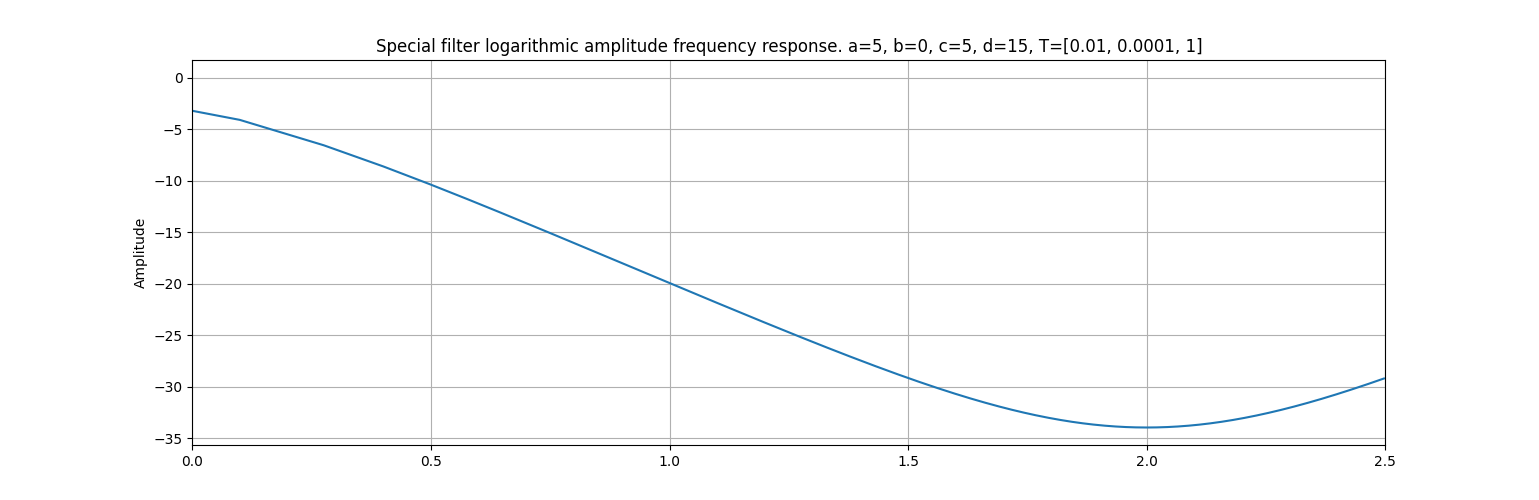
\includegraphics[scale=0.4]{1_fl2_lafr.png}
        \captionsetup{skip=0pt}
        \caption{График логарифмической амплитудно-частотной характеристики фильтра (1).}
        \label{fig:filinlafr21}
    \end{figure}
    \begin{figure}[H]
        \centering
        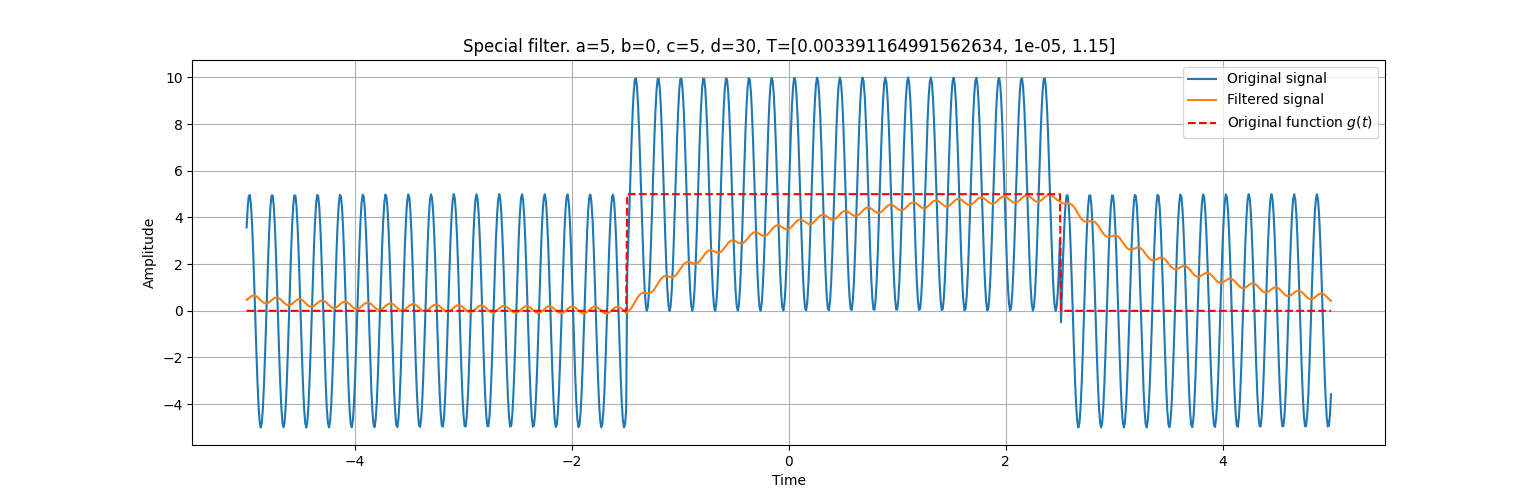
\includegraphics[scale=0.4]{2_fl2.png}
        \captionsetup{skip=0pt}
        \caption{График исходного и фильтрованного сигналов (2).}
        \label{fig:filin22}
    \end{figure}
    \begin{figure}[H]
        \centering
        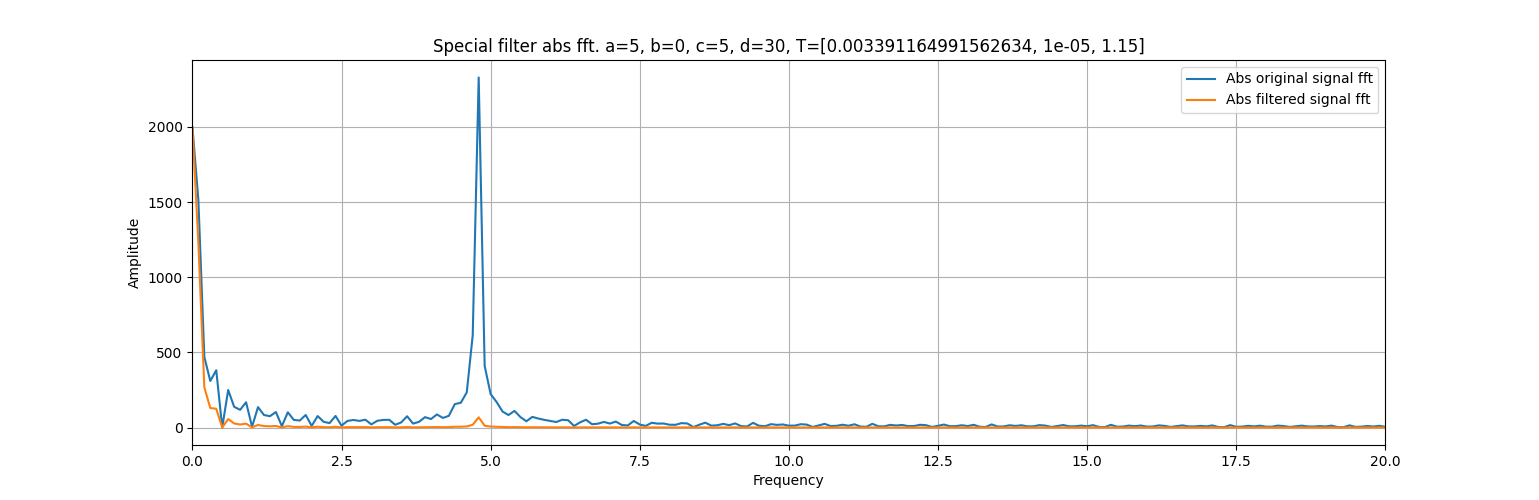
\includegraphics[scale=0.4]{2_fl2_abs.png}
        \captionsetup{skip=0pt}
        \caption{График модулей Фурье-образа исходного и фильтрованного сигналов (2).}
        \label{fig:filinabs22}
    \end{figure}
    \begin{figure}[H]
        \centering
        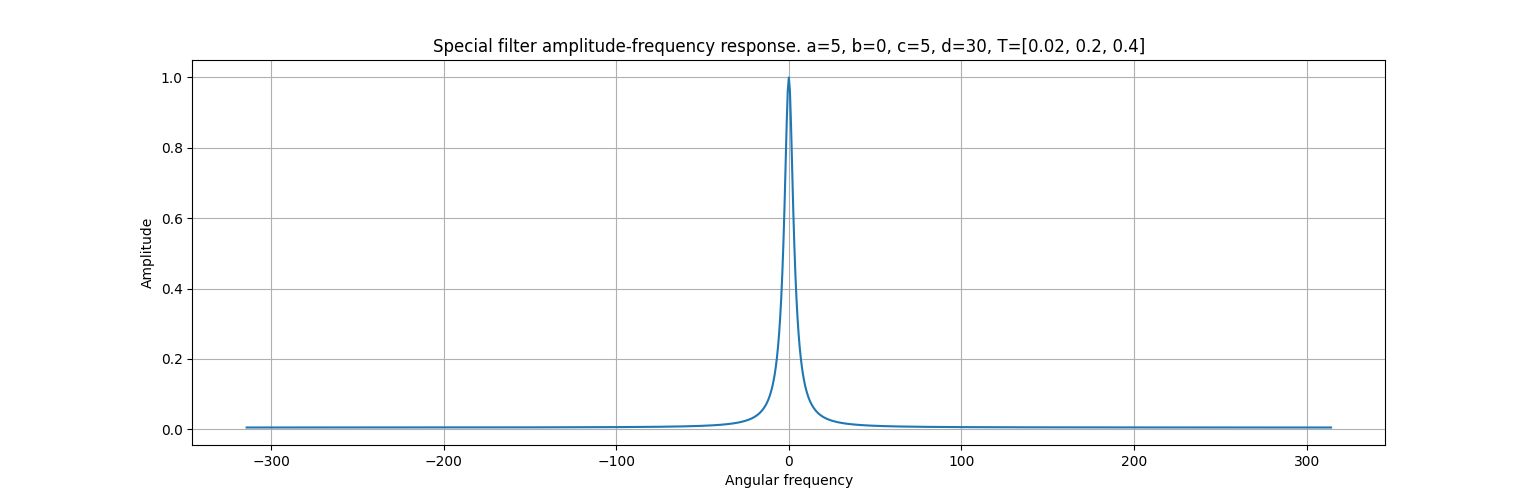
\includegraphics[scale=0.4]{2_fl2_afr.png}
        \captionsetup{skip=0pt}
        \caption{График амплитудно-частотной характеристики фильтра (2).}
        \label{fig:filinafr22}
    \end{figure}
    \begin{figure}[H]
        \centering
        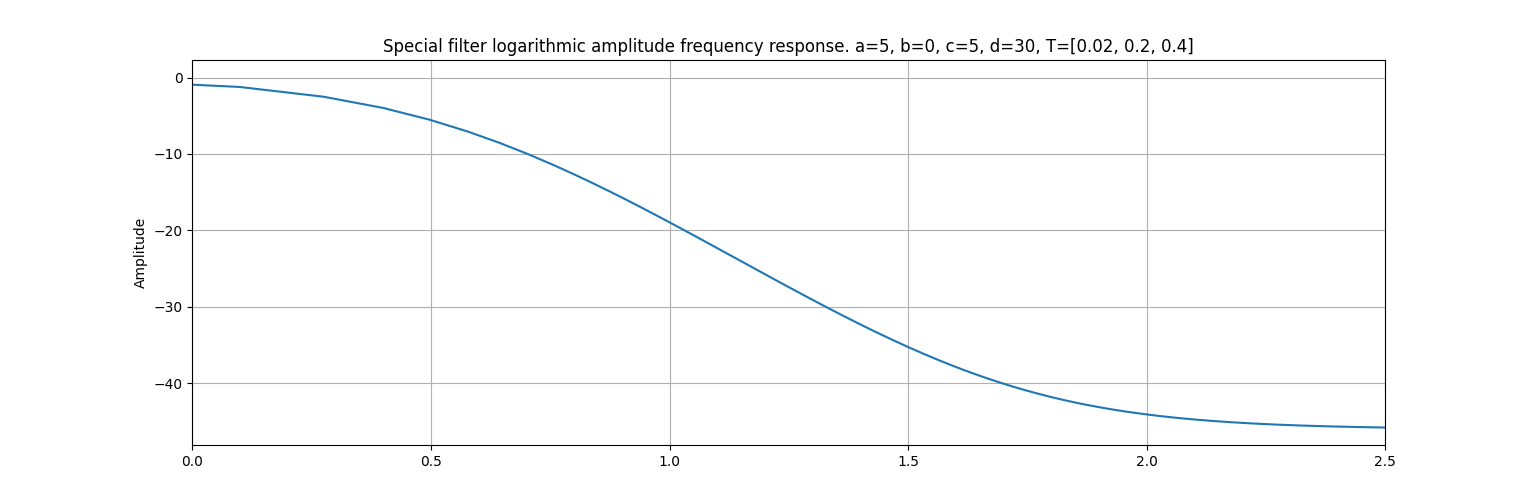
\includegraphics[scale=0.4]{2_fl2_lafr.png}
        \captionsetup{skip=0pt}
        \caption{График логарифмической амплитудно-частотной характеристики фильтра (2).}
        \label{fig:filinlafr22}
    \end{figure}
    \begin{figure}[H]
        \centering
        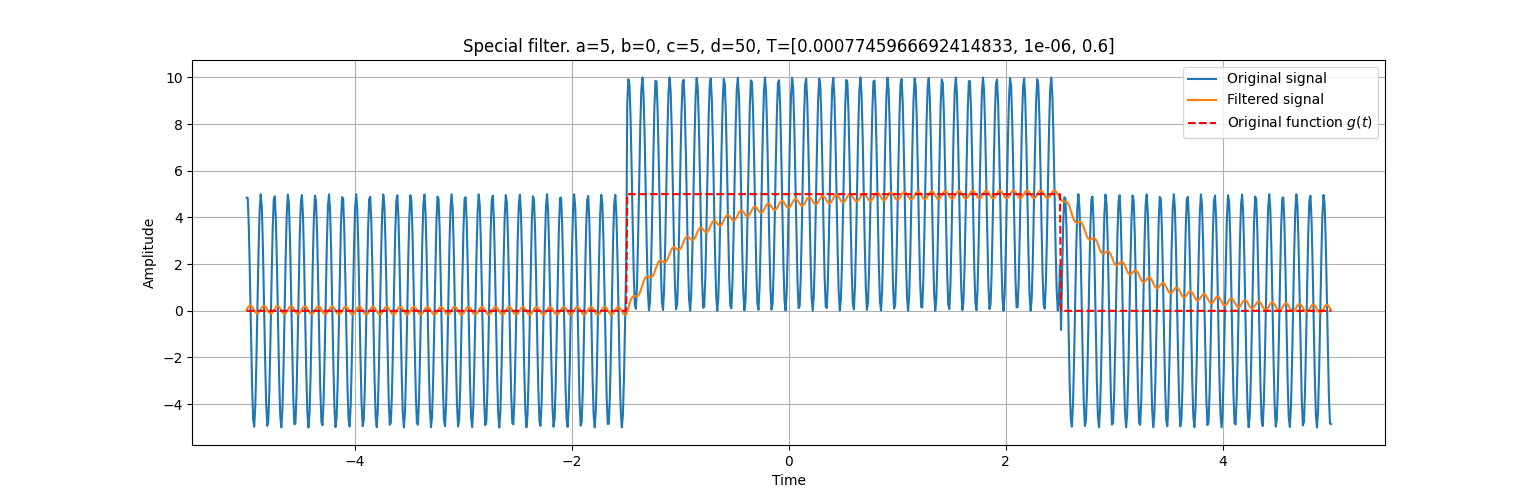
\includegraphics[scale=0.4]{3_fl2.png}
        \captionsetup{skip=0pt}
        \caption{График исходного и фильтрованного сигналов (3).}
        \label{fig:filin23}
    \end{figure}
    \begin{figure}[H]
        \centering
        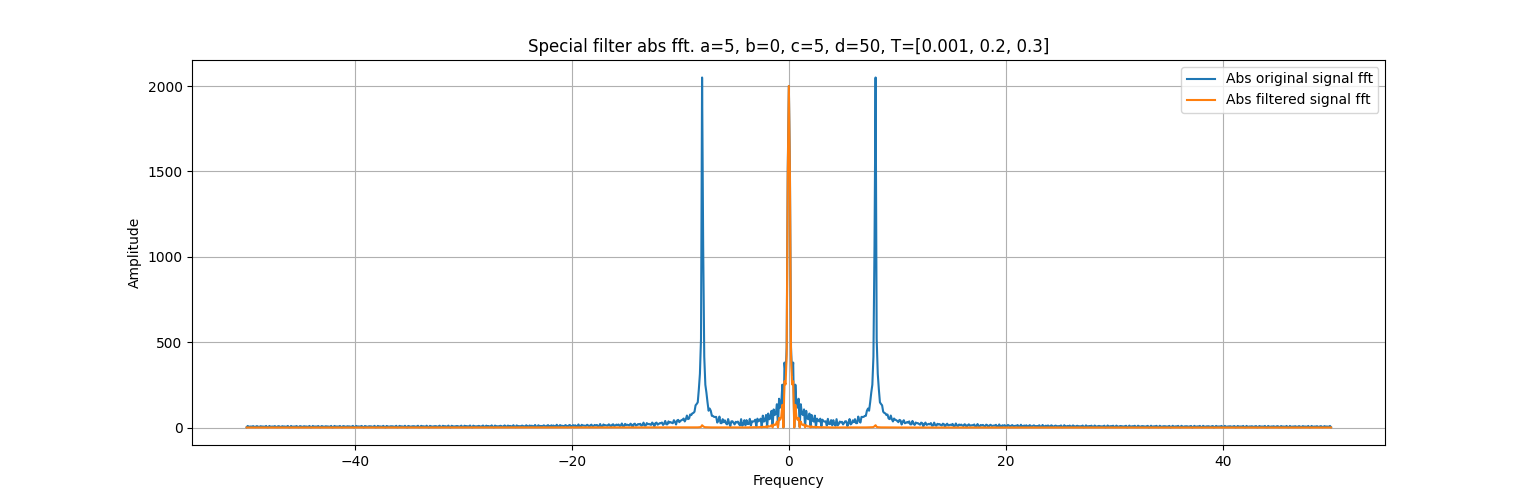
\includegraphics[scale=0.4]{3_fl2_abs.png}
        \captionsetup{skip=0pt}
        \caption{График модулей Фурье-образа исходного и фильтрованного сигналов (3).}
        \label{fig:filinabs23}
    \end{figure}
    \begin{figure}[H]
        \centering
        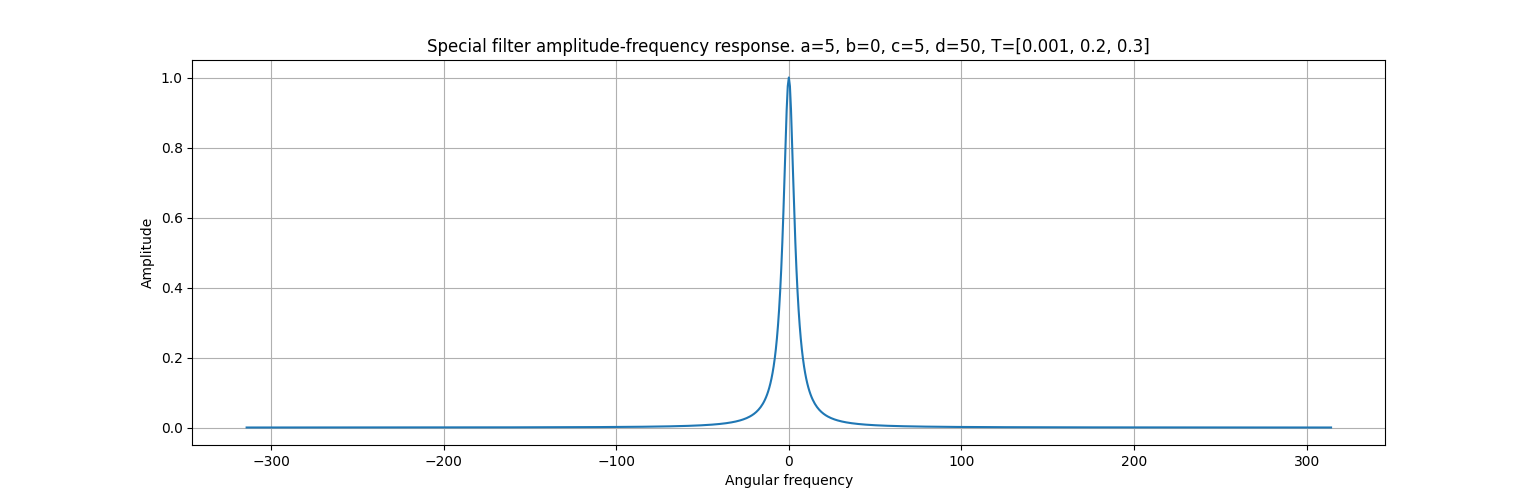
\includegraphics[scale=0.4]{3_fl2_afr.png}
        \captionsetup{skip=0pt}
        \caption{График амплитудно-частотной характеристики фильтра (3).}
        \label{fig:filinafr23}
    \end{figure}
    \begin{figure}[H]
        \centering
        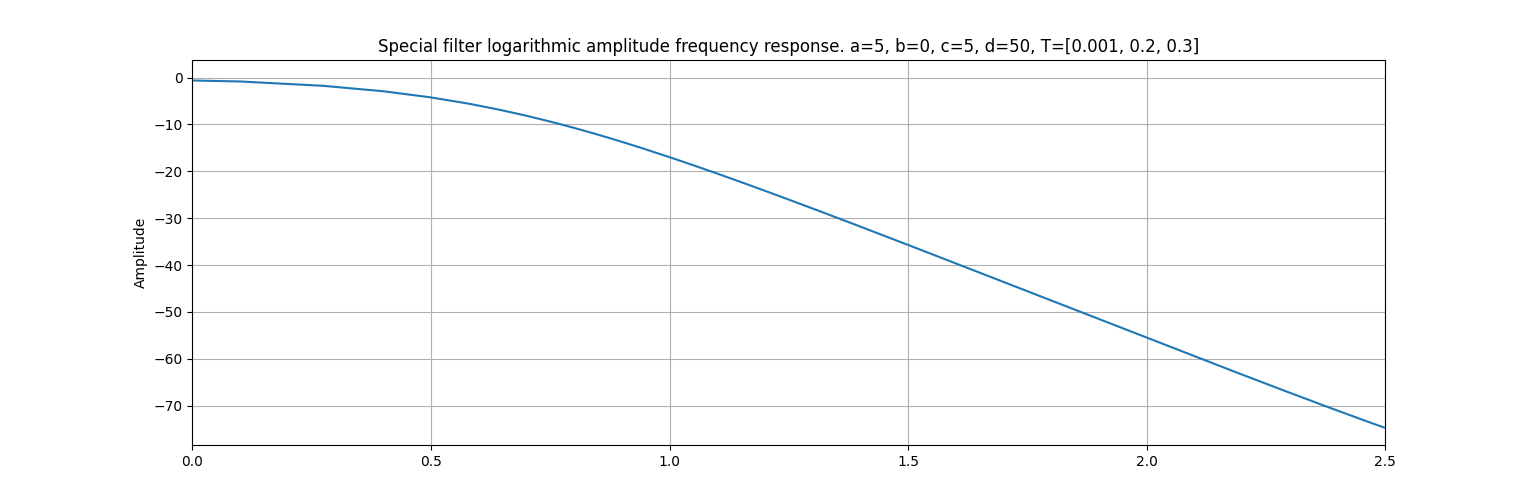
\includegraphics[scale=0.4]{3_fl2_lafr.png}
        \captionsetup{skip=0pt}
        \caption{График логарифмической амплитудно-частотной характеристики фильтра (3).}
        \label{fig:filinlafr23}
    \end{figure}
    \begin{figure}[H]
        \centering
        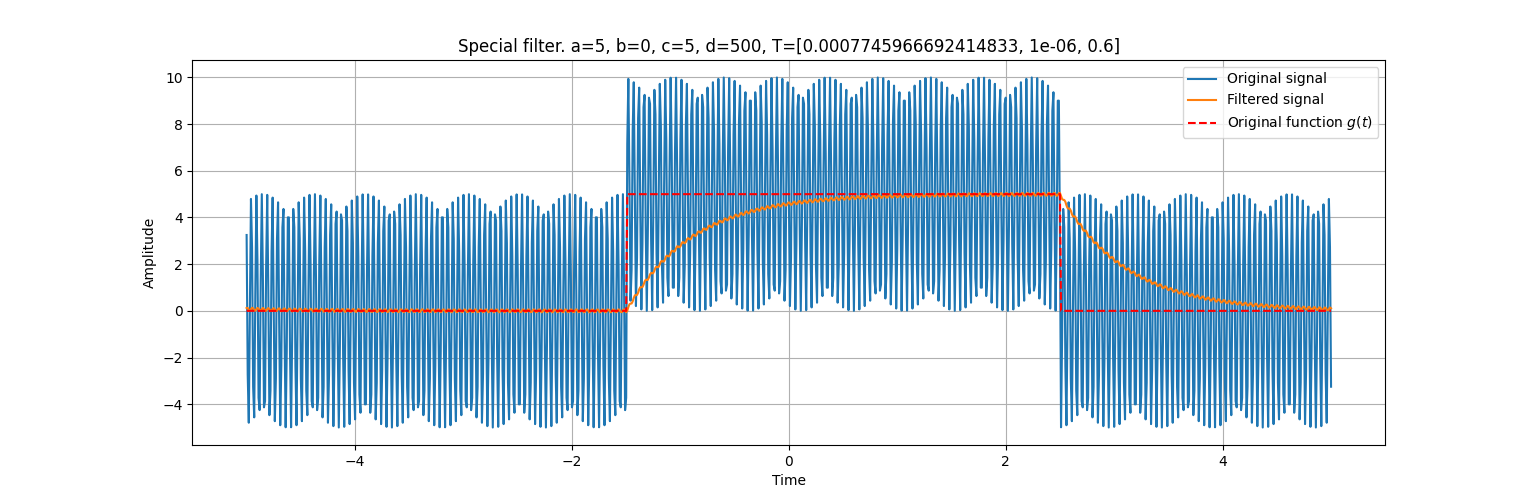
\includegraphics[scale=0.4]{4_fl2.png}
        \captionsetup{skip=0pt}
        \caption{График исходного и фильтрованного сигналов (4).}
        \label{fig:filin24}
    \end{figure}
    \begin{figure}[H]
        \centering
        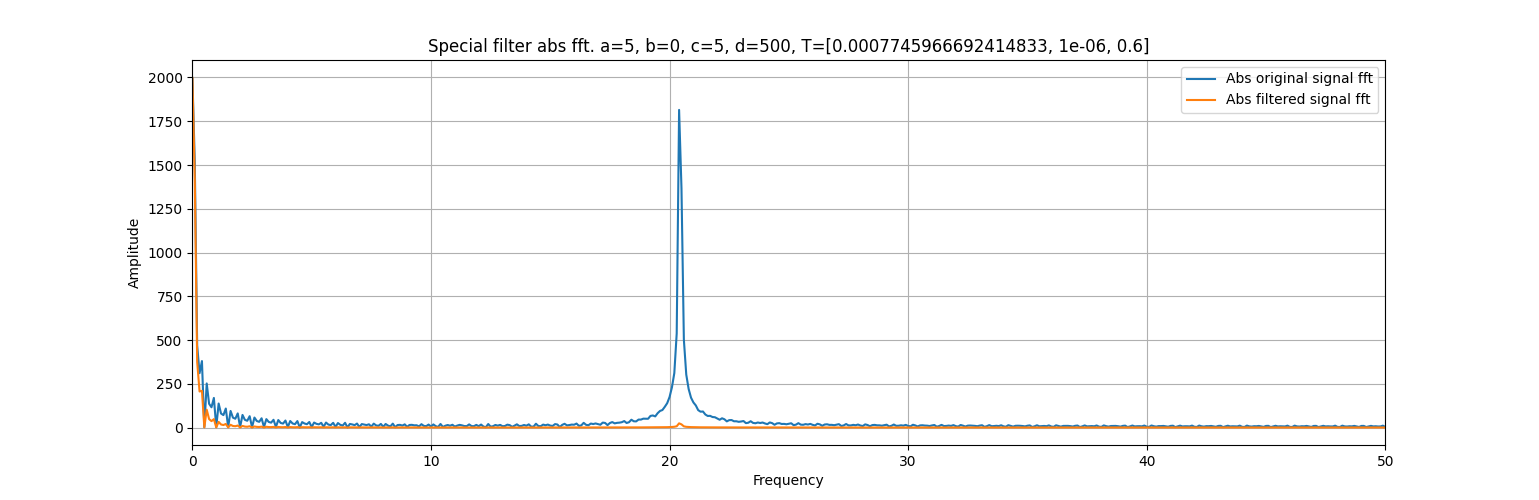
\includegraphics[scale=0.4]{4_fl2_abs.png}
        \captionsetup{skip=0pt}
        \caption{График модулей Фурье-образа исходного и фильтрованного сигналов (4).}
        \label{fig:filinabs24}
    \end{figure}
    \begin{figure}[H]
        \centering
        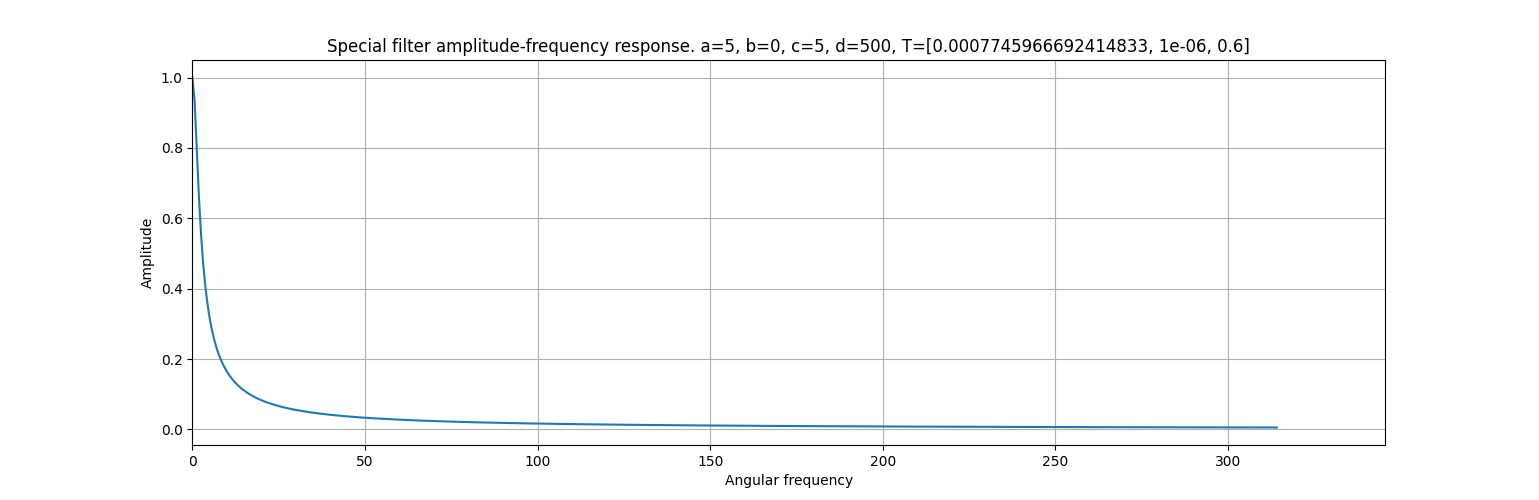
\includegraphics[scale=0.4]{4_fl2_afr.png}
        \captionsetup{skip=0pt}
        \caption{График амплитудно-частотной характеристики фильтра (4).}
        \label{fig:filinafr24}
    \end{figure}
    \begin{figure}[H]
        \centering
        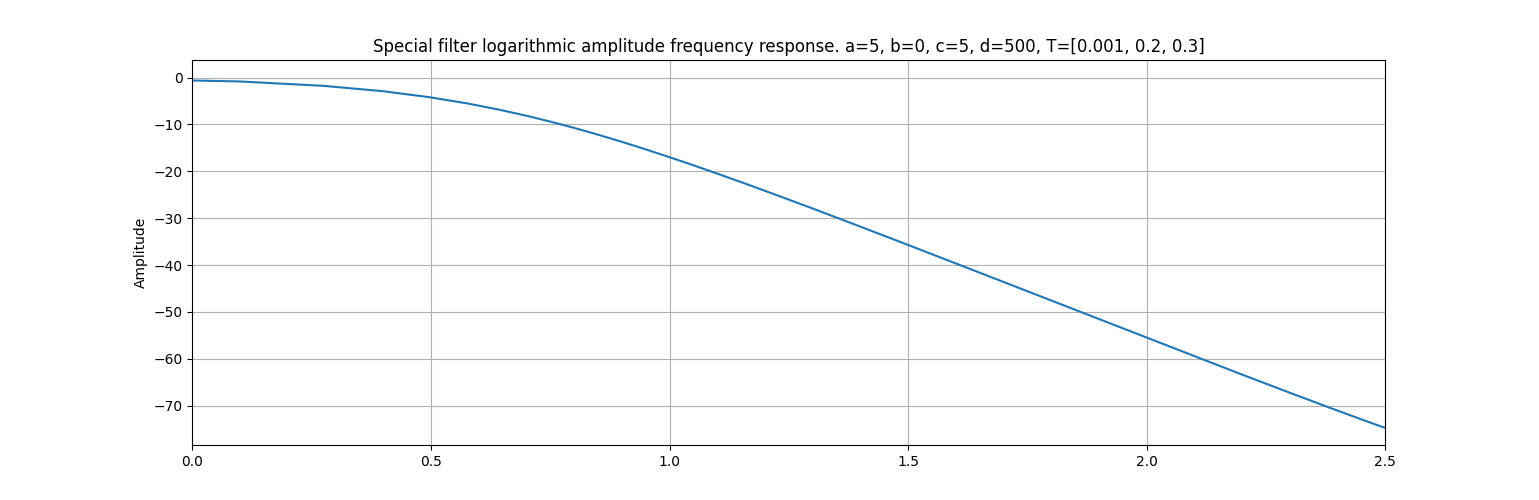
\includegraphics[scale=0.4]{4_fl2_lafr.png}
        \captionsetup{skip=0pt}
        \caption{График логарифмической амплитудно-частотной характеристики фильтра (4).}
        \label{fig:filinlafr24}
    \end{figure}
    \begin{figure}[H]
        \centering
        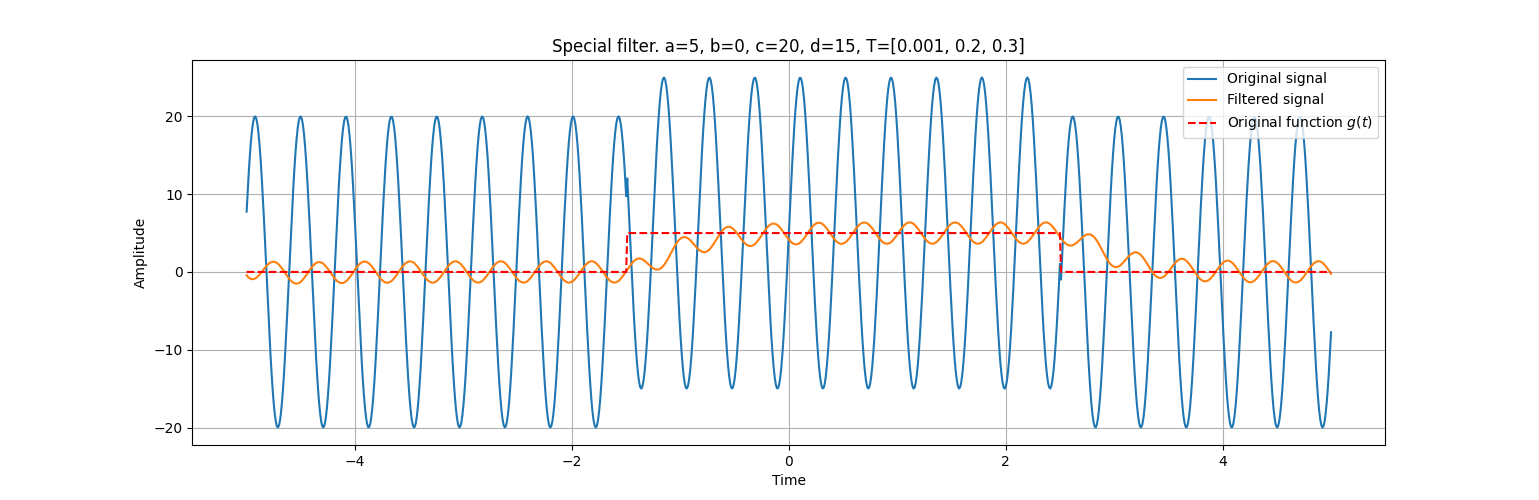
\includegraphics[scale=0.4]{5_fl2.png}
        \captionsetup{skip=0pt}
        \caption{График исходного и фильтрованного сигналов (5).}
        \label{fig:filin25}
    \end{figure}
    \begin{figure}[H]
        \centering
        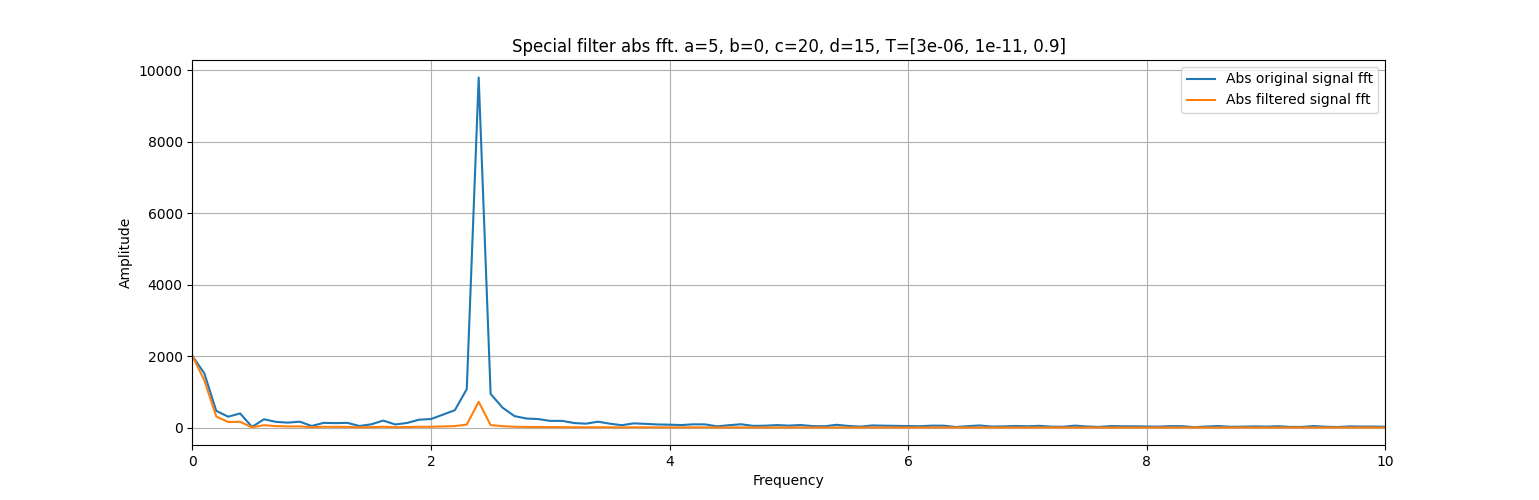
\includegraphics[scale=0.4]{5_fl2_abs.png}
        \captionsetup{skip=0pt}
        \caption{График модулей Фурье-образа исходного и фильтрованного сигналов (5).}
        \label{fig:filinabs25}
    \end{figure}
    \begin{figure}[H]
        \centering
        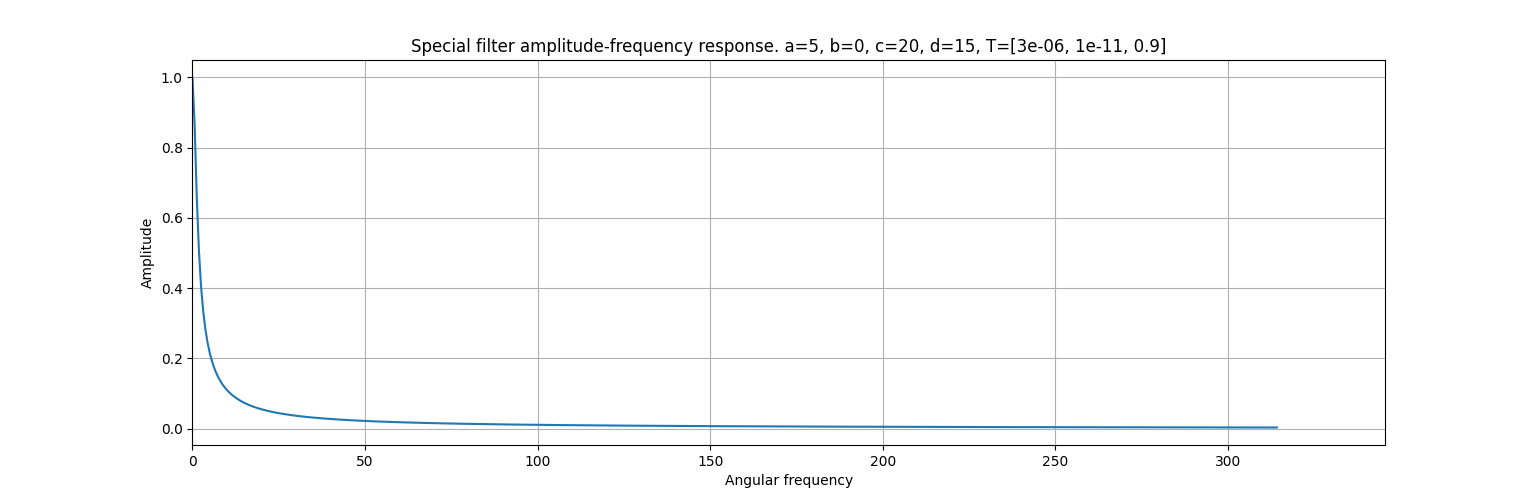
\includegraphics[scale=0.4]{5_fl2_afr.png}
        \captionsetup{skip=0pt}
        \caption{График амплитудно-частотной характеристики фильтра (5).}
        \label{fig:filinafr25}
    \end{figure}
    \begin{figure}[H]
        \centering
        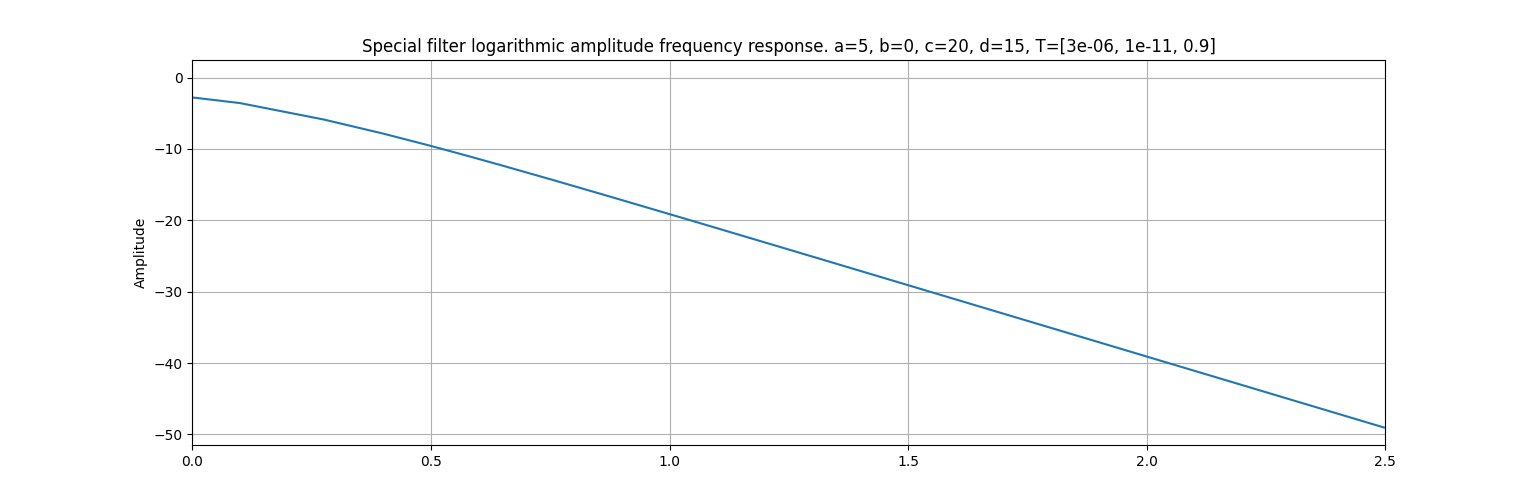
\includegraphics[scale=0.4]{5_fl2_lafr.png}
        \captionsetup{skip=0pt}
        \caption{График логарифмической амплитудно-частотной характеристики фильтра (5).}
        \label{fig:filinlafr25}
    \end{figure}
    \begin{figure}[H]
        \centering
        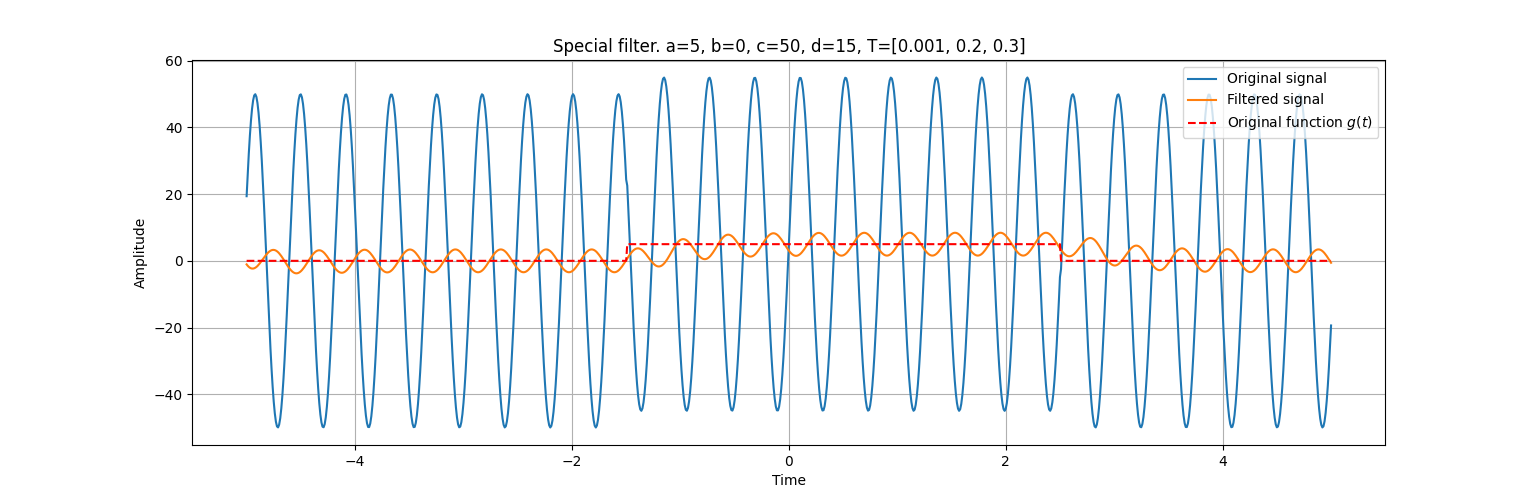
\includegraphics[scale=0.4]{6_fl2.png}
        \captionsetup{skip=0pt}
        \caption{График исходного и фильтрованного сигналов (6).}
        \label{fig:filin26}
    \end{figure}
    \begin{figure}[H]
        \centering
        \includegraphics[scale=0.4]{6_fl2_abs.png}
        \captionsetup{skip=0pt}
        \caption{График модулей Фурье-образа исходного и фильтрованного сигналов (6).}
        \label{fig:filinabs26}
    \end{figure}
    \begin{figure}[H]
        \centering
        \includegraphics[scale=0.4]{6_fl2_afr.png}
        \captionsetup{skip=0pt}
        \caption{График амплитудно-частотной характеристики фильтра (6).}
        \label{fig:filinafr26}
    \end{figure}
    \begin{figure}[H]
        \centering
        \includegraphics[scale=0.4]{6_fl2_lafr.png}
        \captionsetup{skip=0pt}
        \caption{График логарифмической амплитудно-частотной характеристики фильтра (6).}
        \label{fig:filinlafr26}
    \end{figure}
    \begin{figure}[H]
        \centering
        \includegraphics[scale=0.4]{7_fl2.png}
        \captionsetup{skip=0pt}
        \caption{График исходного и фильтрованного сигналов (7).}
        \label{fig:filin27}
    \end{figure}
    \begin{figure}[H]
        \centering
        \includegraphics[scale=0.4]{7_fl2_abs.png}
        \captionsetup{skip=0pt}
        \caption{График модулей Фурье-образа исходного и фильтрованного сигналов (7).}
        \label{fig:filinabs27}
    \end{figure}
    \begin{figure}[H]
        \centering
        \includegraphics[scale=0.4]{7_fl2_afr.png}
        \captionsetup{skip=0pt}
        \caption{График амплитудно-частотной характеристики фильтра (7).}
        \label{fig:filinafr27}
    \end{figure}
    \begin{figure}[H]
        \centering
        \includegraphics[scale=0.4]{7_fl2_lafr.png}
        \captionsetup{skip=0pt}
        \caption{График логарифмической амплитудно-частотной характеристики фильтра (7).}
        \label{fig:filinlafr27}
    \end{figure}


    Исходя из результатов графиков можно сделать вывод, что при увеличении значения параметра $d$ фильтрация
    улучшается. Основная информация об исходном сигнале хранится на нижних частотах, что мы видим на любом
    графике модуля Фурье-образа. Чем меньше значение параметра $d$, тем ближе к нижним частотам расположен
    гармонический шум, проявляющийся в виде двух высоких возрастаниях амплитуд (см. рис. \ref{fig:filinabs21}). Из-за этого при маленьком
    значении параметра $d$ сложно подобрать такие $T_1,\,T_2,\,T_3$, чтобы минимизировать влияние синусоидального
    шума и при этом оставить значимую часть сигнала нетронутой, так как сложнее найти ту частоту среза, выше которой
    фильтр оставит все важные амплитуды и ниже которой полностью уберет амплитуды гармонического шума. В то время как
    при большом значении параметра $d$, при условии отсутствия влияния параметра $b$, выбор коэффициентов, при котором фильтрация
    будет успешна, более разнообразен (см. рис. \ref{fig:filinabs24}). В этом случае выбрать частоту среза проще вследствие
    расширения диапазона ее выбора. В ходе выполнения задания мне удалось получить наилучшую фильтрацию при соотношении
    $T_1<<T_2\approx T_3$.


    Параметр $c$ влияет на амплитуду каждой волны гармонического шума. При увеличении значения параметра $c$ амплитуды увеличиваются
    как во временном пространстве (см. рис. \ref{fig:filin21}, \ref{fig:filin25}, \ref{fig:filin26}), так и в частотном
    (см. рис. \ref{fig:filinabs21}, \ref{fig:filinabs25}, \ref{fig:filinabs26}), а при уменьшении значения -- уменьшаются.
    Данное увеличение амплитуд ухудшает эффективность фильтрации. Придется подобрать такие параметры $T_1,\,T_2,\,T_3$,
    чтобы амплитуды гармонического шума, сильно б\'{о}льшие значимых амплитуд исходного сигнала, ушли под действием фильтра.
    Однако при выборе такой частоты среза высока вероятность, что фильтр не только не сможет достаточно ослабить амплитуды
    синусоидального шума, но и затронет нужные для хорошей фильтрации. Данную проблему хорошо видно на рисунке \ref{fig:filinabs26}.
    При маленьких значениях параметра $c$ фильтрация получается наилучшей (см. рис. \ref{fig:filin27}).


    \subsection{Используемые программы.}
    В ходе выполнения этого задания были использованы некоторые программы, приведенные ранее. В числе новых есть программа,
    реализующая линейные фильтры, рассмотренные в задании.
    \begin{lstlisting}[label=c2, caption={Программа, содержащая реализацию линейных фильтров.}]
    def W_1f(w, T):
        p = 1j * w
        return 1 / (T * p + 1)
    
    def W_2f(w, T_1, T_2, T_3):
        p = 1j * w
        return (T_1 * p + 1) ** 2 / ((T_2 * p + 1) * (T_3 * p + 1))
    \end{lstlisting}


    Добавились функции, необходимые для нахождения АЧХ, ЛАЧХ и пропускания сигнала через фильтр.
    В функции пропуска сигнала через фильтр можно задать параметр shift, он будет необходим позже.
    \begin{lstlisting}[label=c22, caption={Программа для нахождения АЧХ, ЛАЧХ и пропуска сигнала через фильтр.}]
    def fft_flt(u, W, shift=True):
        U = np.fft.fft(u)
        maybe_shifted_U = U
        if shift:
            maybe_shifted_U = np.fft.fftshift(U)
    
        flt_U = W * maybe_shifted_U
        maybe_shifted_flt_U = flt_U
        if shift:
            maybe_shifted_flt_U = np.fft.ifftshift(flt_U)
    
        flt_u = np.fft.ifft(maybe_shifted_flt_U)
        return flt_u, maybe_shifted_flt_U, U
    
    def get_AFR(W):
        return np.abs(W)
    
    def get_LAFR(W):
        return 20 * np.log10(get_AFR(W))
    \end{lstlisting}


    Есть вспомогательная программа для создания исходной функции и исходного сигнала с шумом.
    \begin{lstlisting}[label=help, caption={Программа для создания исходной функции и сигнала с шумом.}]
    def g_func(t, t_1, t_2, a):
        if (t_1 <= t <= t_2): return a
        return 0
    
    def get_g_f(t: list, t_1, t_2, a):
        g_f = []
        for k in range(len(t)):
            g_f.append(g_func(t[k], t_1, t_2, a))
        return g_f
    
    def get_u(g_fs: list, t: list, b, c, d):
        return np.array(g_fs) + b * (np.random.rand(len(t)) - 0.5) + c * np.sin(d * t)
    \end{lstlisting}


    Алгоритм, использующий приведенные ранее программы, расположен ниже.
    \begin{lstlisting}[label=l2, caption={Алгоритм, использующий приведенные ранее программы.}]
    import numpy as np

    import build_func as bf
    import lin_filters as lf
    import fourier_math as fm
    import helper as hr

    def perform(t, v, w, u, a, b, c, d, T, W, W_LOG, g_f=None,
                name='Filter', xl0=None, xl01=None,
                xl1=None, xl2=None, xl3=None,
                xl4=None, xl5=None, xl6=None):
        flt_u, flt_U, U = fm.fft_flt(u, W)
        AFR, LAFR = fm.get_AFR(W), fm.get_LAFR(W_LOG)

        flist1 = [u, flt_u.real]
        flist2 = [abs(np.fft.fftshift(U)), abs(np.fft.fftshift(flt_U))]
        llist1 = ['Original signal', 'Filtered signal']
        llist2 = ['Abs original signal fft', 'Abs filtered signal fft']
        lslist, clist = ['-', '-'], [None, None]
        if g_f is not None:
            flist1.append(g_f)
            llist1.append(r'Original function $g(t)$')
            lslist.append('--')
            clist.append('r')

        bf.build_fs(t, y=flist1, labels=llist1,
              colors=clist, ls=lslist,
              ttl=f'{name}. a={a}, b={b}, c={c}, d={d}, T={T}', 
              xlab='Time', ylab='Amplitude',
              legend=True, xl1=xl0, xl2=xl01)
        bf.build_fs(v, y=flist2, labels=llist2, 
                  ttl=f'{name} abs fft. a={a}, b={b}, c={c}, d={d}, T={T}', 
                  xlab='Frequency', ylab='Amplitude',
                  legend=True, xl1=xl1, xl2=xl2)
        bf.build_f(w, y=AFR,
              ttl=
              f'{name} amplitude-frequency response. a={a}, b={b}, c={c}, d={d}, T={T}',xlab='Angular frequency', 
              ylab='Amplitude',
              xl1=xl3, xl2=xl4)
        bf.build_f(np.log10(w[w > 0]), y=LAFR,
                ttl=
                f'{name} logarithmic amplitude frequency response. a={a}, b={b}, c={c}, d={d}, T={T}',
                ylab='Amplitude',
                xl1=xl5, xl2=xl6)

    T, dt = 10, 0.01
    V, dv = 1 / dt, 1 / T
    t_1, t_2 = -1.5, 2.5

    v_to_w_coeff = 2 * np.pi
    t = np.arange(-T / 2, T / 2 + dt, dt)
    v = np.arange(-V / 2, V / 2 + dv, dv)
    w = v_to_w_coeff * v

    v_log = np.arange(0, V / 2 + dv, dv)
    w_log = v_to_w_coeff * v_log

    perform_W_1, perform_W_2 = True, True

    if perform_W_1:
        a, b, c, d = 1, 0.6, 0, 0.7

        g_fun = hr.get_g_f(t, t_1, t_2, a)
        u = hr.get_u(g_fun, t, b, c, d)

        T_0 = 0.1
        W_1 = lf.W_1f(w, T_0)
        W_1_LOG = lf.W_1f(w_log, T_0)

        perform(t, v, w, u, a, b, c, d, T_0, W_1, W_1_LOG, g_f=g_fun, 
                name='First order linear filter', xl5=0, xl6=2.5)

    if perform_W_2:
        a, b, c, d = 5, 0, 5, 15

        g_fun = hr.get_g_f(t, t_1, t_2, a)
        u = hr.get_u(g_fun, t, b, c, d)

        T_1, T_2, T_3 = 0.001, 0.2, 0.3
        W_2 = lf.W_2f(w, T_1, T_2, T_3)
        W_2_LOG = lf.W_2f(w_log, T_1, T_2, T_3)

        perform(t, v, w, u, a, b, c, d, [T_1, T_2, T_3], W_2, W_2_LOG,
                g_f=g_fun, name='Special filter', xl5=0, xl6=2.5)
    \end{lstlisting}

    
    \section{Задание 3. Сглаживание биржевых данных.}
    В данном задании представим, что мы разрабатываем инвестиционное приложение, в котором должна
    присутствовать функция представления сглаженных графиков котировок акций. При этом степень
    сглаживания должна зависеть от рассматриваемого пользователем временного периода.


    Скачаем с \href{https://www.finam.ru/quote/moex/sber/export/}{данного сайта} файл с данными о
    стоимости акций Сбербанка в период с 21 марта 2018 по 21 марта 2019. Периодичность выберем один день.
    Загрузим данные в Python и применим к данным линейный фильтр первого порядка. Последовательно возьмем
    значения постоянной времени $T$ равной 1 день, 1 неделю, 1 месяц, 3 месяца и 1 год. Представим, что
    во всех месяцах ровно 30 дней, значит за три месяца пройдет 90 дней. Построим красивые сравнительные графики.


    Далее расположены результирующие графики. Синим цветом обозначены исходные данные, оранжевым -- сглаженные.
    По оси абсцисс отложены понедельно даты в период за год, по оси ординат цена закрытия акции. В названии графика
    указаны выбранные параметры шага для частот и временной постоянной.
    \begin{figure}[H]
        \centering
        \includegraphics[scale=0.35]{1_1.png}
        \captionsetup{skip=0pt}
        \caption{График исходных и фильтрованных данных (1).}
        \label{fig:11}
    \end{figure}
    \begin{figure}[H]
        \centering
        \includegraphics[scale=0.35]{1_7.png}
        \captionsetup{skip=0pt}
        \caption{График исходных и фильтрованных данных (1).}
        \label{fig:17}
    \end{figure}
    \begin{figure}[H]
        \centering
        \includegraphics[scale=0.35]{1_30.png}
        \captionsetup{skip=0pt}
        \caption{График исходных и фильтрованных данных (1).}
        \label{fig:30}
    \end{figure}
    \begin{figure}[H]
        \centering
        \includegraphics[scale=0.35]{1_90.png}
        \captionsetup{skip=0pt}
        \caption{График исходных и фильтрованных данных (1).}
        \label{fig:90}
    \end{figure}
    \begin{figure}[H]
        \centering
        \includegraphics[scale=0.35]{1_365.png}
        \captionsetup{skip=0pt}
        \caption{График исходных и фильтрованных данных (1).}
        \label{fig:365}
    \end{figure}
    \begin{figure}[H]
        \centering
        \includegraphics[scale=0.35]{2_1.png}
        \captionsetup{skip=0pt}
        \caption{График исходных и фильтрованных данных (2).}
        \label{fig:112}
    \end{figure}
    \begin{figure}[H]
        \centering
        \includegraphics[scale=0.35]{2_7.png}
        \captionsetup{skip=0pt}
        \caption{График исходных и фильтрованных данных (2).}
        \label{fig:172}
    \end{figure}
    \begin{figure}[H]
        \centering
        \includegraphics[scale=0.35]{2_30.png}
        \captionsetup{skip=0pt}
        \caption{График исходных и фильтрованных данных (2).}
        \label{fig:302}
    \end{figure}
    \begin{figure}[H]
        \centering
        \includegraphics[scale=0.35]{2_90.png}
        \captionsetup{skip=0pt}
        \caption{График исходных и фильтрованных данных (2).}
        \label{fig:902}
    \end{figure}
    \begin{figure}[H]
        \centering
        \includegraphics[scale=0.35]{2_365.png}
        \captionsetup{skip=0pt}
        \caption{График исходных и фильтрованных данных (2).}
        \label{fig:3652}
    \end{figure}


    Как видим, при увеличении параметра $T$ график сглаживается, то есть для более длительного временного периода
    сглаживание становится более склонным к усреднению данных (см. рис. \ref{fig:30}, \ref{fig:90}, \ref{fig:365},
    \ref{fig:3652}). Таким образом сохраняются долгосрочные тренды, а краткосрочные нет. При уменьшении параметра $T$ логика наоборот
    (см. рис. \ref{fig:11}, \ref{fig:17}, \ref{fig:112}, \ref{fig:172}, \ref{fig:302}).


    Шаг времени для частот влияет на степень сглаживания графика при выборе временного периода. Маленький шаг соответствует
    более частым измерениям, сглаживание становится более точным, это может быть полезно для краткосрочных трендов.
    Большой шаг приводит к более грубому сглаживанию, но это может быть полезно для долгосрочных трендов.


    \subsection{Используемые программы.}
    Для выполнения данного задания была написана программа на языке Python. В ней использовались
    некоторые ранее написанные программы. Для нахождения частот была применена функция, реализованная
    в библиотеке numpy. В эту функцию передается шаг по времени, в ходе работы были приведены случаи для
    шагов равных одному дню и одной неделе. Также при использовании моей функции передается параметр shift
    как ложь, так как из-за особенностей работы функции для поиска частот сдвиг для пропускания данных
    через фильтр не нужен.
    \begin{lstlisting}[label=task3, caption={Программа для сглаживания биржевых данных.}]
    import csv
    import numpy as np

    import build_func as bf
    import lin_filters as lf
    import fourier_math as fm

    file = 'fm_lab4/data/SBER_180321_190321.csv'
    find_date = 'DATE'
    find_price = 'CLOSE'
    dates = []
    prices = []
    with open(file) as csv_file:
        csv_reader = csv.reader(csv_file, delimiter=';')
        header = next(csv_reader)
        date_i = 0
        price_i = 0
        for i in range(len(header)):
            if find_date in header[i]:
                date_i = i
            if find_price in header[i]:
                price_i = i

        for row in csv_reader:
            dates.append(row[date_i])
            prices.append(float(row[price_i]))

    date_step = 1
    n = len(dates)
    v = np.fft.fftfreq(n, d=date_step)
    w = 2 * np.pi * v

    T = 1
    W = lf.W_1f(w, T)
    flt_u, flt_U, U = fm.fft_flt(prices, W, shift=False)

    bf.build_fs(dates, [prices, flt_u.real],
                ticks=range(0, len(dates), 7),
                rot=45,
                xlab='Dates',
                ylab=f'Prices ({find_price.lower()})',
                ttl=
                f'First order linear filter, date_step={date_step}, T={T}',
                fz2=8,
                legend=True,
                labels=['Original prices', 'Smoothed prices'])
    \end{lstlisting}
\end{document}